\documentclass[a4paper,fleqn]{cas-sc}

% cas-sc already loads amsmath, amssymb, array, booktabs, graphicx, hyperref,
% xcolor, etc.; only the extra packages our bodies need are added here.
\usepackage[numbers,sort&compress]{natbib}
\usepackage{siunitx}
\usepackage{tabularx}
\usepackage{longtable}
\usepackage{enumitem}
% NB: do NOT load the float package here. The CAS class redefines the figure/table
% environments via expl3 and parses the optional [...] as a key-value list; loading
% float on top hijacks \@float and forces every float to the document end. Placement
% is controlled through the CAS pos key instead (see [pos={!ht}] in the bodies).
\usepackage{placeins}
\graphicspath{{figures/}}

% Macros shared by all three Results bodies (their own \newcommand lines were
% stripped with the section preambles).
\newcommand{\RMSE}{\ensuremath{\mathrm{RMSE}}}
\newcommand{\MAE}{\ensuremath{\mathrm{MAE}}}
\newcommand{\Czon}{\ensuremath{C_{\mathrm{zon}}}}
\newcommand{\Tsupply}{\ensuremath{T_{\mathrm{sup}}}}
\newcommand{\That}{\ensuremath{\widehat{T}}}
% fixed pointer to a float in the separate Supplementary Material PDF
\newcommand{\suppref}[1]{#1}

\begin{document}
\let\WriteBookmarks\relax

\shorttitle{The Fidelity--Utility Paradox in Surrogate-Based RL for HVAC Control}
\shortauthors{Author One et~al.}

\title[mode=title]{The Fidelity--Utility Paradox in Surrogate-Based Reinforcement Learning for HVAC Control}

% ==== TODO authors: replace placeholders with real author data ====
\author[1]{Author One}[orcid=0000-0000-0000-0000]
\cormark[1]
\ead{corresponding.author@example.edu}
\credit{Conceptualization, Methodology, Software, Validation, Formal analysis, Investigation, Writing -- original draft, Writing -- review and editing}
\affiliation[1]{organization={Department, University/Institution},
                city={City},
                postcode={00000},
                country={Country}}
\cortext[cor1]{Corresponding author}
% ==================================================================

\begin{abstract}
Deep reinforcement-learning (RL) controllers for HVAC systems are usually trained against fast neural-network surrogates, on the assumption that a more accurate surrogate is a better training environment. Testing this on the BOPTEST \texttt{bestest\_air} testcase, we report a negative result --- the \emph{fidelity--utility paradox}: the surrogate with the lower predictive error can be the worse environment for policy-gradient search. A grey-box resistance--capacitance surrogate with a neural residual heat-flow head (v3.5) attains a 24-hour rollout RMSE of $0.644\,^{\circ}$C versus $1.557\,^{\circ}$C for a black-box surrogate (v3); yet used directly for training it collapses on the live runtime (maintenance score $m_s = 1.046$, comfort violation $>77\%$), whereas the weaker v3 trains a usable controller ($m_s = 0.073$/$0.095$ on peak/typical windows). Retraining the black-box surrogate at finer resolution makes it \emph{more} accurate yet unusable for training ($m_s > 1.1$), so the paradox tracks a fidelity/smoothing trade-off, not model class alone. We resolve the paradox with a role-separating hybrid: v3 supplies smooth rollout dynamics while a frozen v3.5 acts as a per-step reward-shaping censor. The hybrid provides the best cross-window robustness --- sub-$5\%$ comfort violation on both windows and the lowest typical-window score ($m_s = 0.041$), at ${\sim}85\times$ live-simulator throughput --- and the optimal censor weight is controller-family specific. A transferability study on three hydronic testcases shows the inverse-calibration pipeline generalizes ($60.2$--$87.8\%$ rollout-RMSE reduction; effective zone capacitance re-identified at $1.918\pm0.032\times$ the baseline), whereas frozen-policy transfer is regime-dependent. The contribution is a precise, component-level transferability boundary, not a universal generalization claim.
\end{abstract}

\begin{highlights}
\item A more accurate building surrogate can be a worse RL training environment.
\item Temporal coarse-graining, not black-box structure alone, makes a surrogate useful.
\item A hybrid (black-box rollouts + frozen-twin reward censor) recovers control.
\item The optimal physics-censor weight is controller-family specific.
\item Calibration transfers across testcases; frozen-policy transfer is regime-bound.
\end{highlights}

\begin{keywords}
reinforcement learning \sep HVAC control \sep surrogate model \sep digital twin \sep physics-informed calibration \sep transfer learning \sep BOPTEST
\end{keywords}

\maketitle

\section*{Nomenclature}
\renewcommand{\arraystretch}{1.15}
\begin{longtable}{@{}l l p{0.62\linewidth}@{}}
\textbf{Symbol} & \textbf{Unit} & \textbf{Meaning} \\
\midrule
\endfirsthead
\textbf{Symbol} & \textbf{Unit} & \textbf{Meaning} \\
\midrule
\endhead
\multicolumn{3}{@{}l}{\emph{Thermophysical quantities}}\\
$T_{\mathrm{zone}}$ & \si{\celsius} & zone air temperature \\
$T_{\mathrm{amb}}$ & \si{\celsius} & ambient air temperature \\
$\Tsupply$ & \si{\celsius} & supply-air temperature command \\
$\Czon$ & \si{\joule\per\kelvin} & zone thermal capacitance \\
$R$ & \si{\kelvin\per\watt} & lumped envelope thermal resistance \\
$\eta$ & -- & heating power conversion efficiency \\
$\dot{Q}$ & \si{\watt} & net zone heat flow \\
$P$ & \si{\watt} & total HVAC electrical power \\
$\Delta t$ & \si{\second} & control / integration step (\SI{900}{\second}) \\[2pt]
\multicolumn{3}{@{}l}{\emph{Reinforcement-learning formulation}}\\
$s_t,\,a_t,\,o_t,\,d_t$ & -- & state, action, observation, disturbance at step $t$ \\
$\Phi$ & -- & one-step plant (emulator) transition map \\
$f_\theta,\,g_\phi$ & -- & black-box surrogate (v3) and frozen physical twin (v3.5) \\
$r_t$ & -- & per-step (shaped) reward \\
$\tilde{r}_t$ & -- & hybrid reward with disagreement censor \\
$J(\pi)$ & -- & expected discounted return \\
$\gamma$ & -- & discount factor \\
$w_c,\,w_e,\,w_s$ & -- & comfort / energy / safety preference weights \\
$\hat{A}_t$ & -- & generalized advantage estimate \\
$\rho_t$ & -- & PPO probability ratio \\
$\epsilon$ & -- & PPO clipping parameter \\
$\delta$ & -- & surrogate--twin disagreement penalty \\
$\lambda_T,\,\lambda_P$ & -- & hybrid temperature / power censor weights \\[2pt]
\multicolumn{3}{@{}l}{\emph{Evaluation metrics}}\\
$m_s$ & -- & BOPTEST maintenance score (lower is better) \\
$r_{\mathrm{time}},\,r_{\mathrm{sev}}$ & -- & time-in-violation and severity components of $m_s$ \\
$m_{s,\mathrm{RL}},\,m_{s,\mathrm{PI}}$ & -- & maintenance score of the RL and built-in PI controller \\
$\RMSE_T$ & \si{\celsius} & live closed-loop zone-temperature RMSE \\
CV(\RMSE) & \si{\percent} & coefficient of variation of the RMSE \\
NMBE & \si{\percent} & normalized mean bias error \\
$R^2$ & -- & coefficient of determination \\
Violation & \si{\percent} & fraction of steps outside the comfort band \\
CV & -- & coefficient of variation (std/mean) over seeds \\
$g_a$ & -- & $L_2$ action-gap norm (surrogate vs live) \\
$\Delta m_s$ & -- & live-minus-surrogate $m_s$ transfer gap \\[2pt]
\multicolumn{3}{@{}l}{\emph{Transferability (testcase $k$)}}\\
$\tau_k$ & -- & pre-specified pass threshold $1.25\,m_{s,\mathrm{PI},k}$ \\
$\Delta E_k$ & \si{\percent} & energy change of the RL controller vs PI \\
$G^{\mathrm{RMSE}}_k$ & \si{\percent} & rollout-RMSE improvement after Stage~A/B/C recalibration \\
$\rho_{C,k}$ & -- & re-identified $\Czon$ ratio vs the \texttt{bestest\_air} baseline \\
$\mathcal{A}_k$ & -- & pre-specified actuator adapter \\[2pt]
\multicolumn{3}{@{}l}{\emph{Abbreviations}}\\
BOPTEST & -- & Building Optimization Testing Framework \\
RTE & -- & (BOPTEST) Run-Time Environment \\
DRL / PPO & -- & deep RL / proximal policy optimization \\
GAE & -- & generalized advantage estimation \\
HDRL & -- & hierarchical deep reinforcement learning \\
MORL & -- & multi-objective reinforcement learning \\
POMDP & -- & partially observable Markov decision process \\
RC / ODE & -- & resistance--capacitance / ordinary differential equation \\
PI / RBC / MPC & -- & proportional--integral / rule-based / model predictive control \\
\bottomrule
\end{longtable}

% Introduction -- citations resolved from docs/introduction/ PDFs and wired
% via natbib (\citep) against references.bib; all placeholders resolved.
\section{Introduction}

\subsection{Motivation}
People spend up to 90\% of their time indoors, and buildings account for roughly one third of global final energy use; within them, heating, ventilation, and air-conditioning (HVAC) systems are the single largest consumer~\citep{AlSayed2024Review,Nguyen2024Modelling}. Improving HVAC control is therefore one of the highest-leverage interventions available for building decarbonization, yet it is intrinsically difficult: zone thermodynamics are nonlinear and coupled, and they are driven by time-varying occupancy, weather, and equipment constraints. The controllers used in practice --- proportional--integral (PID) loops and rule-based control (RBC) --- are robust and interpretable but cannot exploit this structure, leaving substantial comfort and energy gains unrealized~\citep{Savino2025ASHRAE,Gao2024Predictive}. Model predictive control (MPC) can exploit it in principle, but it requires an accurate, continuously maintained physical model of each building, which is expensive to identify and brittle under model mismatch~\citep{Hou2024MultiSource}.

Deep reinforcement learning (DRL) is an attractive alternative because it learns a control policy directly from interaction, without an explicit model, and standardized runtime environments such as BOPTEST now make such controllers reproducibly comparable~\citep{Blum2021BOPTEST,AlSayed2024Review}. The obstacle is the sim-to-real deployment gap: policy-gradient algorithms consume millions of environment steps, so training on a live building --- or on a high-fidelity physics simulator stepped through an HTTP interface --- is prohibitively slow and risks sustained comfort violations during exploration~\citep{Wang2025SafeDRL,Hou2024MultiSource}. The community's response is to train the policy against a fast neural-network surrogate of the building, increasingly a physics-informed digital twin (e.g.\ resistance--capacitance or Neural Ordinary Differential Equation models) that generates state transitions orders of magnitude faster than real time~\citep{HouEvins2024,Mshragi2026FastML}. This paradigm rests on an unstated assumption, which we make explicit and test in this work: that a surrogate with higher predictive fidelity is automatically a better environment in which to train a controller.

\subsection{Research gap}
We find that this assumption can fail, and we name the phenomenon the \emph{fidelity--utility paradox}: the surrogate with the lowest multi-step rollout error can be the worst environment for policy-gradient search. When a controller is trained directly on the high-fidelity physical twin, the policy converges to a near bang-bang law (a surrogate-to-live action-gap norm of $2.0$) and fails on the live BOPTEST runtime environment ($m_s>1$, comfort violation above $77\%$), even though that twin is the more accurate offline predictor. We \emph{observe} this action saturation directly; we \emph{hypothesize} that policy-gradient optimizers such as PPO exploit flat-gradient regions of the sharply physics-constrained surrogate, producing actions that do not survive the distribution shift to the live simulator~\citep{RiahiSamani2026OOD}, but the precise mechanism is established only in direction here. Establishing the paradox cleanly is itself non-trivial: two surrogates of different fidelity also differ in their training corpus and time resolution, so any naive fidelity-versus-utility comparison is confounded and must be separated by a controlled decomposition.

A second, orthogonal gap concerns the observation interface and the controller family. HVAC control is a partially observable Markov decision process (POMDP): a small ($5$-dimensional) observation of the instantaneous state is insufficient for preference-conditioned multi-objective control (MORL)~\citep{Byeon2025MaxMinMORL}, which needs forecast and actuation context to disambiguate heating demand~\citep{Gao2024Predictive}. It is also unclear whether a single physics-regularization recipe is universal across controller families, since thermostatic, hierarchical, and multi-objective agents have different loss-surface geometries, so a censor that helps one may over-constrain another. Existing studies seldom separate surrogate predictive fidelity from downstream controller utility, rarely audit the observation interface, and almost never pre-specify cross-testcase transfer hypotheses --- which is precisely the methodological gap this paper addresses.

\subsection{Hypothesis and study design}
We propose a hybrid, role-separating architecture that decouples prediction from training. A compact control-oriented black-box surrogate (v3) supplies smooth, control-friendly Markov rollout dynamics, while an inverse-calibrated physics-informed twin (v3.5), whose zone thermal capacitance $\Czon$ is identified from telemetry, acts as a \emph{frozen per-step reward-shaping censor}: it adds a disagreement penalty to the reward, not a term to the policy loss, so the smooth v3 gradient field is preserved while physically implausible state--action regions are discouraged. To address the POMDP we widen the interface to a $17$-dimensional, forecast-augmented direct-supply-temperature observation, and we evaluate the recipe across three controller families --- thermostatic proximal policy optimization (PPO), hierarchical DRL (HDRL)~\citep{Liao2025HDRL}, and preference-conditioned MORL~\citep{Byeon2025MaxMinMORL}. Finally, the resulting frozen policies are subjected to a pre-specified transferability study on a hydronic family of BOPTEST testcases.

We organize the investigation around four pre-specified, falsifiable hypotheses:
\begin{enumerate}[label=\textbf{H\arabic*.},leftmargin=2.6em]
  \item \emph{Fidelity--utility:} a surrogate with higher predictive fidelity is a better RL training environment.
  \item \emph{Role separation:} using the physical twin as a frozen reward-shaping censor over a smooth black-box rollout recovers the control utility that direct use of the twin destroys.
  \item \emph{Family specificity:} a single physical-censor weight is optimal across controller families.
  \item \emph{Transferability:} the inverse-calibration pipeline and the frozen controller transfer to related hydronic testcases under documented recalibration.
\end{enumerate}
As reported below, H1 and H3 are \emph{falsified}, H2 is supported, and H4 resolves into a component-level boundary --- the calibration pipeline transfers while frozen-controller transfer does not. Each hypothesis and its verdict are bound to a versioned audit anchor, so that every outcome was predictable but not predicted before the corresponding runs.

\subsection{Results summary}
The evidence answers these questions concretely. Calibrated v3.5 reduces the 24-hour rollout RMSE to $0.644\,^{\circ}$C (versus $1.557\,^{\circ}$C for v3), yet used directly it yields $m_s=1.046$ live; the predictively weaker v3 yields a usable controller ($m_s=0.073$/$0.095$). The hybrid backend recovers the best cross-window robustness profile ($m_s=0.087$/$0.041$, violation below $5\%$ on both windows) while sustaining $85.0\times$ the BOPTEST throughput. The optimal disagreement weight is controller-family specific ($\lambda_{\mathrm{temp}}=0.10$ for thermostatic PPO, $\lambda_{\mathrm{temp}}=0$ for HDRL and the $17$D MORL). On the hydronic family, the inverse calibration transfers ($60.2$--$87.8\%$ rollout-RMSE reduction; $\Czon$ re-identified at $1.918\pm0.032$ times the source value), whereas frozen-policy transfer is regime-dependent.

\subsection{Contributions}
This paper makes three commit-anchored, version-locked contributions, organized as the project's three evidence blocks:
\begin{enumerate}
  \item \textbf{Inverse-calibration pipeline and a matched-corpus decomposition (Block 1).} A Stage~A/B/C inverse-calibration protocol for the physical twin, with a controlled experiment attributing the predictive-fidelity gain to a $74.6\%$ data-resolution component and a $25.4\%$ physical-calibration component, so the calibration claim is real but bounded.
  \item \textbf{The fidelity--utility paradox and its hybrid resolution (Block 2).} Empirical evidence that a higher-fidelity physical surrogate is the worse direct RL training environment, resolved by a hybrid role assignment (v3 dynamics + frozen-v3.5 reward-shaping censor); the censor strength is shown to be controller-family specific, and the MORL controller beats the built-in PI baseline in mean (with the $N=5$ seed variance reported honestly).
  \item \textbf{A commit-anchored, version-locked transferability study (Block 3).} Across a hydronic family of testcases, the identified zone capacitance $\Czon$ transfers as a near-uniform structural invariant (rollout-RMSE improvement up to $88\%$), while zero-shot transfer of the frozen controller fails or passes only with an energy penalty --- establishing a precise component-level transferability boundary rather than a universal generalization claim.
\end{enumerate}
The remainder of this paper is organized as follows. Section~\ref{sec:related} reviews related work; Section~\ref{sec:methodology} details the methodology; Section~\ref{sec:setup} describes the experimental setup; Sections~\ref{sec:results1-digital-twin}, \ref{sec:results2-control}, and~\ref{sec:results3-transfer} present Results~I, II, and III; Section~\ref{sec:discussion} discusses the findings; and Section~\ref{sec:conclusion} concludes.

\section{Related Work}\label{sec:related}
\subsection{Deep and multi-objective reinforcement learning for HVAC control}
Deep reinforcement learning (DRL) has become the dominant learning-based approach
to supervisory HVAC control, yet the review of \citet{AlSayed2024Review} finds
that only a minority of studies reach real-building deployment and that agents are
typically trained on a single testbed with limited exposure to exogenous
variation. Concrete controllers illustrate both the promise and this narrowness:
phasic policy-gradient control improves adaptivity and convergence on a
building-energy task \citep{Nguyen2024Modelling}; low-level multi-zone DRL has been
benchmarked directly against ASHRAE Guideline~36 sequences \citep{Savino2025ASHRAE};
and multi-agent formulations address energy management under chance constraints
\citep{Deng2025MultiAgent} or couple DRL to IoT telemetry for context-aware
operation \citep{Alotaibi2025ContextAware}. Because comfort and energy are
competing objectives, HVAC control is naturally multi-objective: hierarchical DRL
decomposes the problem across timescales to trade indoor-air-quality against
consumption \citep{Liao2025HDRL}, while the broader multi-objective RL (MORL)
literature studies preference-conditioned policies and their convergence
guarantees \citep{Byeon2025MaxMinMORL}. What this body of work does not isolate is
whether a single training recipe holds \emph{across} these controller families, or
how the choice of training environment --- rather than the algorithm --- shapes the
resulting policy; both are central questions in this paper.
\subsection{Surrogate and physics-informed models for building control}
Because high-fidelity building simulators are too slow to supply the millions of
interactions that data-driven controllers require, a now-standard response is to
replace --- or accelerate --- the physical model with a learned surrogate.
\citet{HouEvins2024} formalize this practice into a reproducible protocol for
developing and evaluating neural-network surrogate models of building energy
behaviour, establishing reporting and justification levels that we adopt as an
audit standard in this work. At the extreme of the throughput axis,
\citet{Mshragi2026FastML} implement a random-forest surrogate as an FPGA hardware
accelerator, reaching over $1.67$ million predictions per second so that an
evolutionary optimizer can re-tune airflow and supply-temperature set-points in
real time. Such fast surrogates are what make learning-based supervisory control
tractable at building scale: multi-agent deep reinforcement learning has been
applied to smart-building energy management under chance constraints
\citep{Deng2025MultiAgent}, and context-aware reinforcement-learning controllers
coupled to IoT telemetry have been reported to jointly improve energy efficiency
and thermal comfort \citep{Alotaibi2025ContextAware}. In every case the surrogate
or fast model is the substrate on which the controller is trained and tuned.
These surrogates span a fidelity spectrum, from purely data-driven black-box
networks to physics-informed digital twins --- resistance--capacitance or Neural
ODE structures whose parameters carry physical meaning --- and the protocol of
\citet{HouEvins2024} is, to date, oriented toward the predictive accuracy of such
models rather than their suitability as a training environment.

This body of work, however, optimizes the surrogate almost exclusively along two
axes --- predictive accuracy and inference throughput --- and treats the
\emph{use} of that surrogate as a downstream concern. In parallel, the
reinforcement-learning literature studies how training data should be
\emph{collected} from a simulator: \citet{Mayor2025Parallelized} analyze how
on-policy parallelized data collection shapes the optimization stability and final
performance of PPO agents, while \citet{Radac2025OnlineRL} examine the software
mechanics of interleaving environment stepping with learning updates for
near-real-time online RL. What neither strand asks is whether a surrogate that is
\emph{more accurate} as a predictor is thereby a \emph{better environment} in
which to train a controller. We make exactly this question explicit and answer it
in the negative (Section~\ref{sec:results2-control}): the surrogate's predictive
fidelity and its downstream control utility are distinct, and can even be
opposed --- a gap the accuracy-and-throughput framing of the surrogate literature
leaves unexamined.
\subsection{Distribution shift and transfer in learning-based control}
A policy is only as good as the states it was trained to see, and two failure
modes follow. The first is informational: a controller acting on an instantaneous
observation cannot anticipate demand, and augmenting the state with predictive
(forecast) information has been shown to improve both cost and comfort in
office-building HVAC control \citep{Gao2024Predictive}. The second is
distributional: policies optimised on a fixed simulator or offline dataset degrade
when the deployment distribution differs, the out-of-distribution problem
catalogued for offline RL by \citet{RiahiSamani2026OOD}. The standard remedy for
the cost of re-training is transfer learning --- \citet{Hou2024MultiSource}, for
example, transfer pre-trained DRL parameters across building zones and weather
conditions to cut training time --- but they also show that an ill-chosen source
domain degrades performance, so transfer is neither automatic nor uniformly
beneficial. This motivates treating cross-testcase transfer as a hypothesis to be
\emph{tested} rather than assumed, which is the stance of our transferability study
(Section~\ref{sec:results3-transfer}).

\medskip
\noindent\textbf{Positioning.} Across these strands the literature optimises the
controller, the surrogate, and the transfer procedure largely in isolation, and
evaluates each on the axis most natural to it --- algorithmic return, predictive
accuracy, or training-time reduction. The assumption that ties them together ---
that a more accurate or higher-fidelity model is a better basis for control, and
that a recipe tuned on one controller or testcase carries over --- is rarely made
explicit and almost never pre-specified and falsified. This paper isolates that
assumption: it separates surrogate predictive fidelity from downstream control
utility (Section~\ref{sec:results1-digital-twin}--\ref{sec:results2-control}),
tests whether one physics-regularisation recipe holds across controller families
(Section~\ref{sec:results2-control}), and audits cross-testcase transfer against
pre-specified anchors (Section~\ref{sec:results3-transfer}).

\section{Methodology}\label{sec:methodology}
This section gives the formal, self-contained statement of the control problem,
the three surrogate models, the controller families, and the evaluation protocol.
The detailed numerical instantiation of every quantity defined here --- network
sizes, calibrated parameters, hyperparameters, and measured scores --- is reported
with the corresponding evidence in Sections~\ref{sec:results1-digital-twin}--\ref{sec:results3-transfer};
here we fix notation and cite the methods on which the design rests.

\subsection{Reference environment}\label{ssec:m-env}
The plant is a single-zone building emulator with electric heating, drawn from the
BOPTEST family of Modelica-based test cases \citep{Blum2021BOPTEST,Wetter2014Modelica}
and served to the controller through BOPTEST's uniform HTTP interface
\citep{Arroyo2021GymBOPTEST}. Formally the emulator is a continuous-time
dynamical system whose latent thermal state evolves under a scalar heating command
$a_t\in[0,1]$ and an exogenous disturbance stream $d_t$ (ambient weather,
solar gain, occupancy, and time-varying comfort set-points). We interact with it
at a fixed control period $\Delta t = \SI{900}{\second}$ (15 minutes), yielding the
discrete-time transition $s_{t+1}=\Phi(s_t,a_t,d_t)$ that all surrogates are trained
to approximate. The primary test case is \texttt{bestest\_air}; a hydronic family of
related test cases is held out for the transferability study (Section~\ref{sec:results3-transfer}).

\subsection{Problem formulation}\label{ssec:m-pomdp}
Because the controller never observes the full latent state, control is a partially
observable Markov decision process (POMDP)
$\langle \mathcal{S},\mathcal{A},\mathcal{O},\Phi,R,\gamma\rangle$, where the agent
receives an observation $o_t=h(s_t,d_t)\in\mathcal{O}$ and selects $a_t\sim\pi(\cdot\mid o_t)$
so as to maximise the expected discounted return
\begin{equation}
J(\pi)=\mathbb{E}_{\pi}\!\left[\sum_{t=0}^{T-1}\gamma^{t}\,r_t\right],
\qquad
r_t = -\big(w_{\mathrm{c}}\,c_t + w_{\mathrm{e}}\,e_t\big),
\label{eq:m-return}
\end{equation}
with $c_t$ a thermal-discomfort term, $e_t$ the heating energy over the step, and
$w_{\mathrm{c}},w_{\mathrm{e}}$ trade-off weights. Partial observability is the
methodological reason a five-dimensional instantaneous observation is insufficient
and a forecast-augmented observation is required \citep{Gao2024Predictive}; the
exact channel sets are given in Section~\ref{sec:results2-control}. For
\emph{evaluation} (as opposed to training) we score deployed controllers with the
duration-and-severity maintenance score
\begin{equation}
m_s = r_{\mathrm{time}} + r_{\mathrm{sev}},
\label{eq:m-ms}
\end{equation}
the time-in-violation plus violation-severity metric of \citet{Wang2025SafeDRL};
lower is better and $m_s>1$ marks an unacceptable controller. This separation of a
shaped training reward~\eqref{eq:m-return} from an unshaped safety score~\eqref{eq:m-ms}
follows standard practice in safe reinforcement learning \citep{Garcia2015SafeRL}.

\subsection{Surrogate model design}\label{ssec:m-surrogate}
All three surrogates are fast approximations of $\Phi$ used as the training
environment in place of the slow emulator, in the model-based / Dyna tradition of
learning a model and planning or training a policy against it
\citep{Sutton1991Dyna,Hafner2025Dreamer}. They differ in how much building physics
is hard-wired into their structure.

\subsubsection{Control-oriented surrogate v3}
v3 is a compact black-box neural one-step predictor
$\hat{s}_{t+1}=f_\theta(s_t,a_t,d_t)$, trained by supervised minimisation of a
multi-step rollout error so that long-horizon trajectories --- not just one-step
residuals --- stay accurate. Its design goal is not maximal predictive accuracy but
a \emph{smooth, well-conditioned} response surface for policy-gradient search; the
architecture and parameter count are reported in Section~\ref{sec:results1-digital-twin}.

\subsubsection{Physically informed surrogate v3.5 and Stage A/B/C calibration}
v3.5 replaces the black box with a grey-box resistance--capacitance (RC) thermal
network whose unmodelled heat flow is supplied by a neural residual head. It is an
ODE-structured grey-box surrogate --- a continuous-time RC balance, in the spirit
of Neural ODEs \citep{Chen2018NeuralODE} and classical RC building identification
\citep{Bunning2020RC,Berthou2014RC,Bacher2011RCIdentification,Picard2017WhiteBox},
but integrated discretely by an explicit Euler step at the control period
$\Delta t$ rather than by an adaptive ODE solver. Writing the zone capacitance as
$\Czon$ and a lumped envelope resistance as $R$, the core balance is
\begin{equation}
\Czon\,\frac{\mathrm{d}T}{\mathrm{d}t}
= \frac{T_{\mathrm{amb}}-T}{R} + \eta\,a_t\,\dot{Q}_{\max} + q_d,
\label{eq:m-rc}
\end{equation}
with $\eta\,a_t\,\dot{Q}_{\max}$ the delivered heating power and $q_d$ aggregated
disturbance gains (the neural residual head). Embedding this conservation law in the
network makes it physics-informed in the sense of
\citet{Raissi2019PINN,Karpatne2017TheoryGuided,Willard2022PIML}, so its parameters
are physically interpretable; we nonetheless treat $\Czon$ as an \emph{effective}
thermal capacitance under the chosen surrogate structure --- a lumped parameter
that may absorb unmodelled fast dynamics --- rather than a direct measurement of
zone air capacitance. The parameters are recovered by a staged inverse calibration
(Stages~A/B/C) in the spirit of staged grey-box calibration
\citep{Bacher2011RCIdentification}, and the identifiability of $\Czon$ is checked
with a Fisher/Laplace confidence interval; the staged protocol and the resulting
calibrated values are detailed in Section~\ref{sec:results1-digital-twin}.

\subsubsection{Hybrid surrogate and reward-shaping censor}
The hybrid backend assigns the two models orthogonal roles: v3 supplies the smooth
rollout dynamics, while a \emph{frozen} v3.5 acts as a per-step reward-shaping
censor. Training uses the shaped reward
\begin{equation}
\tilde{r}_t = r_t - \lambda_T\,\delta^{T}_t - \lambda_P\,\delta^{P}_t,
\label{eq:m-hybrid}
\end{equation}
where the disagreement terms are the per-step $L_1$ (absolute) distances between the
one-step predictions of the rollout surrogate $f_\theta$ (v3) and the frozen twin
$g_\phi$ (v3.5), separately for the zone temperature and the HVAC power channel,
\begin{equation}
\delta^{T}_t = \big|\, f^{T}_\theta(s_t,a_t,d_t) - g^{T}_\phi(s_t,a_t,d_t)\,\big|\ [\si{\celsius}],
\qquad
\delta^{P}_t = \big|\, f^{P}_\theta(s_t,a_t,d_t) - g^{P}_\phi(s_t,a_t,d_t)\,\big|\ [\si{\watt}],
\label{eq:m-delta}
\end{equation}
with no squaring, normalisation, or clipping. The two censor weights differ in scale
because they multiply a temperature residual (in \si{\celsius}) and a power residual
(in \si{\watt}); for the thermostatic controller $\lambda_T = 0.10$ and
$\lambda_P = 5\times10^{-5}$. Crucially, $g_\phi$ is evaluated \emph{forward only}
and its outputs are detached, so the censor enters the \emph{reward}, never the
policy loss or the surrogate gradient: the well-conditioned v3 gradient field of
Section~\ref{ssec:m-surrogate} is preserved while physically implausible
state--action regions are discouraged --- a model-based shaping that keeps the
benefits of Dyna-style training \citep{Sutton1991Dyna} without inheriting the
sharp gradients of the physical twin. The swept values of $\lambda_T$ per
controller family are given in Section~\ref{sec:results2-control}.

\subsection{Controller families}\label{ssec:m-controllers}
All policies are optimised with proximal policy optimization (PPO)
\citep{Schulman2017PPO} using generalized advantage estimation
\citep{Schulman2016GAE} and the Stable-Baselines3 implementation
\citep{Raffin2021SB3}; PPO maximises the clipped surrogate objective
\begin{equation}
L^{\mathrm{CLIP}}(\theta)=\mathbb{E}_t\!\left[\min\!\big(\rho_t(\theta)\,\hat{A}_t,\;
\operatorname{clip}(\rho_t(\theta),1-\epsilon,1+\epsilon)\,\hat{A}_t\big)\right],
\qquad \rho_t(\theta)=\frac{\pi_\theta(a_t\mid o_t)}{\pi_{\theta_{\mathrm{old}}}(a_t\mid o_t)},
\label{eq:m-ppo}
\end{equation}
with $\hat{A}_t$ the GAE advantage. We evaluate the surrogate recipe across three
controller families of increasing structure: (i) a \emph{thermostatic} PPO agent on
a compact observation; (ii) a \emph{hierarchical} DRL controller (HDRL) that
decomposes control across timescales, in the options/feudal tradition
\citep{Bacon2017Options,Nachum2018HIRO} as recently applied to year-round HVAC
operation \citep{Liao2025HDRL}; and (iii) a \emph{preference-conditioned}
multi-objective controller (MORL) that conditions on a comfort--energy preference
vector \citep{Yang2019MORL,Roijers2013MOSurvey,Hayes2022MOSurvey,Byeon2025MaxMinMORL}
and acts on the forecast-augmented observation. The exact observation and action
spaces of each family are specified in Section~\ref{sec:results2-control}.

\subsection{Evaluation protocol and transferability methodology}\label{ssec:m-eval}
Surrogate predictive fidelity is reported with the ASHRAE-style calibration
statistics CV(\RMSE) and NMBE over multi-step rollouts, the standard accuracy
measures for calibrated building models \citep{Bacher2011RCIdentification}.
Downstream control utility is reported with the maintenance score~\eqref{eq:m-ms}
\citep{Wang2025SafeDRL}, the comfort-violation fraction, and heating energy,
each benchmarked against BOPTEST's built-in baseline controller. Because a policy
trained on a surrogate is deployed on a different (live) system, the central
methodological risk is dataset/distribution shift \citep{Quinonero2009DatasetShift};
we therefore always report the \emph{live}-emulator score, never only the
surrogate-internal score. For transferability we adopt a commit-anchored, version-locked
protocol: each hypothesis (H1--H4 of Section~\ref{sec:related}), pass threshold, and
recalibration adapter is fixed in a version-locked source-control commit
\emph{before} the corresponding runs, and these commits are publicly available in
the open-source repository (Section~\ref{sec:conclusion}, Data availability),
providing timestamped, immutable verifiability of the analysis plan in lieu of
formal pre-registration on an external registry. Cross-test-case transfer is realised through a light recalibration adapter
rather than assumed zero-shot, following the evidence that transfer is
source-dependent \citep{Hou2024MultiSource}. Controller scores are reported with
seed statistics wherever repeated-seed runs are available: MORL is evaluated over
the five fixed seeds $\{42,43,44,45,46\}$, whereas the thermostatic PPO and HDRL
targeted-window experiments are deterministic single-seed mechanistic comparisons,
a limitation stated explicitly in Section~\ref{ssec:b3lim}. The full statistical
and audit protocol is given in Section~\ref{sec:setup} and the results in
Sections~\ref{sec:results1-digital-twin}--\ref{sec:results3-transfer}.

\section{Experimental Setup}\label{sec:setup}
\subsection{Testbeds, serving layer, and runtime}\label{ssec:s-testbed}
All controllers are evaluated on the Building Optimization Testing Framework
(BOPTEST), an open, Modelica-based runtime that exposes building emulators through
a uniform HTTP interface for simulation-based benchmarking of control strategies
\citep{Blum2021BOPTEST,Wetter2014Modelica,Arroyo2021GymBOPTEST}; we use the
\texttt{bestest\_air} testcase as the primary environment and a hydronic family
(\texttt{bestest\_hydronic} variants) for the transferability study of
Section~\ref{sec:results3-transfer}. The controller interacts with the plant at a
fixed \SI{15}{\minute} control period through the same HTTP contract regardless of
which of four interchangeable backends sits behind it: the live BOPTEST runtime,
the black-box surrogate v3, the physically informed surrogate v3.5, or the hybrid.
This common interface is what makes the surrogate-versus-live comparison clean ---
only the dynamics backend changes. On a single commodity workstation the surrogate
backends run \numrange{85.0}{114.2}$\times$ faster than the live BOPTEST RTE HTTP
loop, which is what renders policy-gradient training (millions of environment
steps) tractable without a GPU; the exact per-backend throughput is reported in
Section~\ref{sec:results2-control}.

\subsection{Data generation and preprocessing}\label{ssec:s-data}
Surrogate training and calibration use three purpose-built corpora, generated by
exciting the emulator under scripted heating schedules across cool, heat, mixed,
ramp, and pulse scenarios: a \emph{canonical} v3 corpus ($51{,}200$ samples at
\SI{1}{\hour} resolution), a \emph{15-minute exploration} corpus ($48{,}384$
samples at \SI{900}{\second}), and a v3.5 \emph{calibration} corpus ($10{,}744$
samples at \SI{900}{\second}); the full corpus specification is tabulated in
Section~\ref{sec:results1-digital-twin}. The deliberate pairing of a one-hour and a
fifteen-minute corpus is not incidental: it is the instrument that lets the
matched-corpus ablation of Block~1 attribute the predictive-fidelity gain to data
resolution versus physical calibration, rather than confounding the two. All
channels (zone temperature, heating command, and exogenous disturbances) are
normalised before training, and trajectories are windowed for multi-step rollout
supervision.

\subsection{Training and calibration workflow}\label{ssec:s-train}
The black-box surrogate v3 ($8{,}482$ parameters) is fit by supervised
multi-step rollout regression on the canonical corpus. The physically informed
v3.5 is identified by the staged inverse calibration of
Section~\ref{ssec:m-surrogate} \citep{Bacher2011RCIdentification}: Stage~A/B/C
recover the RC parameters from the calibration corpus, yielding a zone capacitance
$\Czon = \SI{4.413e5}{\joule\per\kelvin}$ ($+5.1\%$ relative to the
$\SI{4.200e5}{\joule\per\kelvin}$ physical prior) subject to a capacitance floor
$c_{\min}=\SI{5e4}{\joule\per\kelvin}$. Controllers in all three families are then
trained with PPO \citep{Schulman2017PPO} using Stable-Baselines3
\citep{Raffin2021SB3}; the hybrid configuration additionally loads the frozen v3.5
as the reward-shaping censor of Eq.~\eqref{eq:m-hybrid}. Hyperparameters and the
censor-weight sweep are reported with the corresponding results in
Section~\ref{sec:results2-control}.

\subsection{Statistical and audit protocol}\label{ssec:s-audit}
Controller scores are reported with seed statistics where repeated-seed runs are
available: the MORL family is evaluated over $N=5$ fixed seeds with the
seed-to-seed variance stated explicitly, while the thermostatic PPO and HDRL
targeted-window experiments are deterministic single-seed mechanistic comparisons
(Section~\ref{ssec:b3lim}); every controller is benchmarked against BOPTEST's
built-in PI controller; the predictive-fidelity and control-utility metrics
themselves (CV(\RMSE), NMBE, and the maintenance score $m_s$ of
Eq.~\eqref{eq:m-ms} \citep{Wang2025SafeDRL}) are defined once in
Section~\ref{ssec:m-eval} and not repeated here. The transferability study follows
a commit-anchored, version-locked discipline: each hypothesis (H1--H4) is bound to a
versioned audit anchor committed \emph{before} the corresponding runs, so that an
outcome can falsify a claim rather than merely illustrate it. The scripts,
configurations, and artefact manifests that regenerate every number, figure, and
table are listed under Data availability.

\paragraph{Software environment.} Controllers are trained with Stable-Baselines3
2.1.0 (PyTorch) under Python~3.11; the reference environment is the
\texttt{ibpsa/project1-boptest} BOPTEST Docker image, driven through its HTTP API.
The MORL runs use the five fixed seeds $\{42,43,44,45,46\}$, while the
thermostatic-PPO and HDRL targeted-window comparisons are deterministic
single-seed (seed~42) evaluations. The released
repository pins these package versions, the controller and surrogate checkpoints,
the per-seed configurations, and the random seeds, so that every result can be
reproduced from the archived artefacts.

% ===== Results sections (auto-generated bodies; sections 5, 6, 7) =====
% Auto-generated by docs/build_integrated_paper.py -- do not edit by hand.
% Standalone scaffolding (preamble, nomenclature, limitations, conclusion,
% \setcounter) stripped for \input into the combined manuscript.
\section{Digital-Twin Fidelity and the RL-Utility Paradox}
\label{sec:results1-digital-twin}

This Results~I section reports the Block~1 evidence chain exactly in the order used by the reproducibility roadmap. Its purpose is to establish the empirical foundation for the central claim of the article: predictive fidelity and reinforcement-learning training utility are related but not identical objectives. Block~1 proves the digital-twin side of this claim. It shows how a compact control-oriented v3 surrogate and a physically informed v3.5 surrogate differ in architecture, calibration, data resolution, rollout accuracy, and runtime feasibility. The downstream question---whether the more accurate twin is also the better PPO training environment---is intentionally carried forward to Results~II, where live BOPTEST controller transfer is evaluated. The mechanism invoked there is a \emph{distributional shift} between the surrogate's training distribution and the live closed-loop state distribution that a trained policy induces~\citep{RiahiSamani2026OOD,Quinonero2009DatasetShift}: a more faithful surrogate can present a sharper response surface that policy-gradient search exploits into a control law which does not survive transfer to the live plant.

\paragraph{Roadmap boundary and artifact chain.}
\label{ssec:block1-roadmap-boundary}

Block~1 asks whether the surrogate family is credible as a fast, physically interpretable digital twin. It does not yet ask whether a controller trained on that surrogate transfers to the live BOPTEST RTE. The executed roadmap path is:
\begin{enumerate}
  \item collect and train the v3 direct-\Tsupply{} surrogate using \texttt{evaluation/run\_block1.py collect-data} and \texttt{v3-train};
  \item prepare the 15-minute corpus and run v3.5 Stage~A/B/C inverse calibration using \texttt{prepare-15min} and \texttt{v35-calibrate --preset canonical};
  \item retrain v3 on the same 15-minute corpus using \texttt{v3-train-15min} to bound the calibration claim;
  \item build the Hou-and-Evins reporting tables and speed benchmark using \texttt{build-reports} and \texttt{speed-benchmark}.
\end{enumerate}



\subsection{Direct Supply-Temperature Control Interface}
\label{ssec:block1-direct-tsup}

All Block 1 surrogates share a single \emph{direct supply-temperature} (direct-\Tsupply{}) control parameterization: the policy commands the supply-air temperature setpoint directly, and the surrogate consumes that setpoint as a boundary condition instead of modelling the upstream valve/coil actuator chain. The two-dimensional action \(a=(a_0,a_1)\in[-1,1]^2\) maps affinely to physical commands,
\begin{equation}
  \Tsupply = 18 + \tfrac{a_0+1}{2}\,(35-18)~[^\circ\mathrm{C}],
  \qquad
  u_{\mathrm{fan}} = \tfrac{a_1+1}{2}\in[0,1],
  \label{eq:action-map}
\end{equation}
and every surrogate exposes the same transition signature
\begin{equation}
  f:\ (T_{\mathrm{zone}},T_{\mathrm{amb}},h,d,a_0,a_1)\ \longmapsto\ (\That_{t+1},\widehat{P}_{t+1}),
  \label{eq:tsup-signature}
\end{equation}
with \(\widehat{P}\ge 0\) enforced by a Softplus output and capped at \(P_{\max}=5500~\mathrm{W}\). A single adapter wraps four interchangeable backends behind \eqref{eq:tsup-signature}---legacy v3, raw v3.5, calibrated v3.5, and the hybrid pairing---which is what makes the like-for-like fidelity comparisons in this section well posed: only the internal dynamics change, never the control interface or the observation map.

\begin{table}[pos={!ht}]
\centering
\small
\caption{Modelling assumptions of the direct-\Tsupply{} control interface.}
\label{tab:tsup-assumptions}
\begin{tabularx}{\linewidth}{lX}
\toprule
Assumption & Statement \\
\midrule
Actuator abstraction & Supply-air temperature is commanded directly; valve/coil dynamics are not modelled beyond the Stage A latency term. \\
Command bounds & \(\Tsupply\in[18,35]\,^\circ\)C; fan command \(u_{\mathrm{fan}}\in[0,1]\). \\
Power non-negativity & \(\widehat{P}=\mathrm{Softplus}(\cdot)\ge 0\), capped at \(P_{\max}=5500\)~W. \\
State support & Zone and ambient temperatures normalized to \([-1,1]\) over \([15,35]\) and \([-10,40]\,^\circ\)C. \\
Interface invariance & All four backends obey \eqref{eq:tsup-signature}; only the internal dynamics differ. \\
\bottomrule
\end{tabularx}
\end{table}

\subsection{Control-Oriented Surrogate Architecture (v3)}
\label{ssec:block1-v3}

The v3 surrogate is a compact control-oriented direct-\Tsupply{} model. Its role is not to be the most accurate long-horizon forecaster; its role is to provide smooth and fast rollout dynamics for downstream PPO experiments. In contrast, v3.5 is a physics-informed extension whose Stage B parameter is interpretable as the zone thermal capacitance \(\Czon\); embedding thermodynamic structure directly into the learned model follows the physics-informed reinforcement-learning paradigm~\citep{Hedayat2025PINN}.

\begin{table}[pos={!ht}]
\centering
\small
\caption{Block 1 data corpora referenced by the roadmap.}
\label{tab:block1-corpora}
\begin{tabularx}{\linewidth}{lrrXX}
\toprule
Dataset & Rows & Step (s) & Policy mix & Scenario mix \\
\midrule
v3 canonical corpus & 51,200 & 3600 & cool, heat, mixed, random & autumn, spring, summer, winter \\
v3.5 calibration corpus & 10,744 & 900 & hdrl, thermostatic & peak\_heat\_window, typical\_heat\_window \\
15-min exploration corpus & 48,384 & 900 & cool, heat, mixed, pulse, random, thermostatic\_noise & autumn, spring, summer, winter \\
\bottomrule
\end{tabularx}
\end{table}



\begin{table}[pos={!ht}]
\centering
\scriptsize
\caption{Architecture and calibration summary for the two Block 1 surrogate roles.}
\label{tab:architecture-summary}
\begin{tabularx}{\linewidth}{lXXXX}
\toprule
Surrogate & Role & Architecture / physics & Corpus & Training or calibration protocol \\
\midrule
v3 direct-TSup & Fast control-oriented rollout dynamics & 8D dual-head MLP: HeatFlowNetV2 (7,105 params, LayerNorm/Tanh/residual), PowerNetV2 (1,377 params, Tanh/Softplus); total 8,482 params & 51,200 hourly transitions & AdamW, lr=1e-3, batch=256, epochs=500 \\
v3.5 calibrated & Physics-informed predictive twin & RC-NeuralODE backbone with positive C\_zon reparameterization and residual temperature/power heads & 10,744 prepared 15-min transitions & Stage A latency/bias; Stage B 120 epochs; Stage C 60+80 epochs; C\_zon=4.413e5 J/K \\
\bottomrule
\end{tabularx}
\end{table}

The v3 transition model is
\begin{align}
  \Delta \That_{t+1} &= f_{\theta,T}(x_t), &
  \widehat{P}_{t+1} &= f_{\theta,P}(x_t), &
  \That_{t+1} &= T_t+\Delta \That_{t+1}.
\end{align}
It is trained by a multi-horizon supervised objective with a physical-consistency penalty,
\begin{equation}
  \mathcal{L}_{v3}
  = \sum_{k\in\{1,2,4\}} \frac{1}{N}\sum_{i}\big(\That_i(t{+}k)-T_i(t{+}k)\big)^2
  + \lambda_{\mathrm{phys}}\,\mathrm{ReLU}\!\big(|\Delta\That|-\Delta T_{\max}\big),
  \label{eq:v3-loss}
\end{equation}
where the multi-step term (horizons of 1, 2, and 4 transitions) enforces short-horizon rollout consistency and the penalty discourages physically implausible single-step jumps. The update \(\That_{t+1}=T_t+\Delta\That_{t+1}\) carries \emph{no} explicit time step: the learned increment is a per-transition quantity, the design choice revisited in Section~\ref{ssec:block1-stepsize}.



The canonical v3 checkpoint is the early-stopped optimum of a 215-epoch supervised run: the best validation epoch is 185, at which the held-out one-step temperature fit reaches \(R^2=0.991\). This single-step score is deliberately optimistic relative to the multi-step rollout error in Section~\ref{ssec:block1-predictive-diagnostics}, which is the metric that actually governs whether the surrogate can substitute for BOPTEST.



The v3 input vector is intentionally low-dimensional. It keeps only the thermal state, outdoor disturbance, cyclic time embedding, and direct-\Tsupply{} action coordinates required by the control problem. The action coordinate \(a_0\in[-1,1]\) is mapped to an 18--35~$^\circ$C supply-temperature command --- a direct supply-temperature setpoint interface of the kind shown effective for DRL-based room HVAC control~\citep{Sun2024DirectTSup} --- and the power head is constrained through a non-negative output transform. These choices make v3 a control-oriented surrogate rather than a generic black-box forecaster. Its full hyperparameters and layer shapes are listed in Supplementary Table~\suppref{S4}.



\subsection{Physics-Informed Twin and Inverse Calibration (v3.5)}
\label{ssec:block1-v35-calibration}

Unlike the purely black-box v3 head, the v3.5 surrogate is built on a first-principles lumped-capacity zone balance with a single effective parameter, the zone thermal capacitance \(\Czon\),
\begin{equation}
  \Czon\,\frac{\mathrm{d}T_{\mathrm{zone}}}{\mathrm{d}t} = \dot{Q}(x;\phi),
  \qquad \dot{Q}(x;\phi)=q_{\mathrm{scale}}\,q_\phi(x),
  \label{eq:rc-ode}
\end{equation}
where \(\dot{Q}(x;\phi)\) is a learned net heat-flow head (\(q_{\mathrm{scale}}=3000\)~W). HVAC input, envelope coupling, and internal gains are absorbed into \(\dot{Q}\) through the feature vector \(x\); there is no separately parameterized \(1/R\) term. With control step \(\Delta t\), \eqref{eq:rc-ode} is integrated by an explicit Euler step,
\begin{equation}
  \That_{t+1} = \mathrm{clip}\!\Big(T_t + \Delta t\,\frac{\dot{Q}(x;\phi)}{\Czon},\ T_{\min},\,T_{\max}\Big).
  \label{eq:rc-euler}
\end{equation}
To keep the inverse problem well posed, \(\Czon\) is not a free scalar but a positively reparameterized one,
\begin{equation}
  \Czon = c_s\big(\mathrm{softplus}(\rho) + c_{\min}/c_s\big),
  \qquad \Czon \ge c_{\min} = 5\times10^4~\mathrm{J/K},
  \label{eq:czon-reparam}
\end{equation}
with \(\rho\) the learnable log-parameter and \(c_s=10^5\) a fixed scale; this guarantees a physically positive capacitance throughout optimization. Because \(\Czon\) is a property of the building rather than of the data-generating policy, it is expected to remain meaningful across testcases, which is what makes the inverse identification below worthwhile.

The roadmap builds the canonical v3.5 artifact by two sequential preset runs. Stage~A aligns telemetry and removes latency/bias artifacts. Stage~B identifies \(\Czon\) on excitation-rich windows. Stage~C then calibrates residual heads while preserving the physical parameter. The first preset, \texttt{block1\_15min\_episodeaware}, performs the temperature-side inverse identification: Stage~B runs for 120 epochs and Stage~C runs for 60 epochs. The second preset, \texttt{block1\_15min\_power\_head\_only}, loads the first summary JSON, freezes \(\Czon\), skips Stage~B, and refines only the power residual head for 80 epochs. This two-pass structure is why the power-head JSON reports \texttt{stage\_b\_epochs\_ran=0}; it is not a missing calibration step.

Stage A estimates a one-step latency compensation, a temperature bias correction of -0.105~$^\circ$C, and a postprocessed temperature RMSE of 0.238~$^\circ$C. Stage B uses the top-excitation subset: 403 of 8058 training rows at excitation quantile 0.95. This filtering is important because \(\Czon\) is identifiable mainly during transients, not quasi-steady operation.





Formally, Stage B is a maximum-a-posteriori estimate of the single physical scalar,
\begin{equation}
  \hat C_{\mathrm{zon}}
  = \arg\min_{C}\ \sum_{i\in\mathcal{E}}\big(\That_i(C)-T_i\big)^2
  + \frac{1}{2\sigma_p^2}\big(C-C^{\mathrm{prior}}\big)^2,
  \label{eq:stageb-map}
\end{equation}
where \(\mathcal{E}\) is the excitation subset and the quadratic term is a weak Gaussian prior centred on \(C^{\mathrm{prior}}\). The excitation filter is justified by identifiability: in quasi-steady operation the sensitivity \(\partial\That/\partial C\to 0\), so steady windows carry almost no information about \(\Czon\) and would merely pull the estimate back to the prior. Restricting \(\mathcal{E}\) to the top-excitation transients (403 of 8058 rows) concentrates the identification where \(\partial\That/\partial C\) is large, which is why the mean excitation score on \(\mathcal{E}\) is several times the corpus mean (Table~\suppref{S7}).

The intermediate Stage~B estimate is \(\Czon=4.413\times10^5~\mathrm{J/K}\), and the relative update over the physical prior is
\begin{equation}
  \eta_C =
  \frac{\Czon^{\mathrm{final}}-\Czon^{\mathrm{prior}}}{\Czon^{\mathrm{prior}}}
  = 0.0506,
\end{equation}
where \(\Czon^{\mathrm{final}}=4.413 \times 10^5~\mathrm{J/K}\). The update remains inside the prior physical plausibility band.

Beyond the point estimate, two complementary uncertainty checks apply. The optimizer is well conditioned (over the final 20 Stage~B epochs the \(\Czon\) trajectory is stable to within \(\pm1,005\)~J/K, 0.23\%). More importantly, a Laplace/Fisher identifiability interval --- obtained from the local curvature of the one-step temperature SSE with respect to \(\Czon\) (residual heads fixed) over the high-excitation transients (\(n=1838\)) --- gives a \(1\sigma\) uncertainty of 6.6\% and a 95\% interval \([3.845,\,4.980]\times10^5\)~J/K. The \(+5.1\%\) data-driven update therefore sits within roughly one standard error of the prior: \(\Czon\) is identifiable with a moderate, honestly bounded signal rather than a tightly pinned value. Physically, the identified capacitance corresponds to an equivalent thermal mass of \(\Czon/c_{p,\mathrm{air}}\approx439\)~kg of air (\(c_{p,\mathrm{air}}=1005~\mathrm{J\,kg^{-1}K^{-1}}\)), or roughly 366~m\(^3\) of equivalent air volume at \(\rho=1.2~\mathrm{kg\,m^{-3}}\). This is the expected order of magnitude for the \texttt{bestest\_air} zone augmented by the effective thermal mass of its internal surfaces, which is exactly why the data-driven update over the air-only prior is small (\(+5\%\)) rather than large.

\medskip\noindent\textbf{Physical-consistency audit.} As a final check we probe the learned dynamics directly: sweeping the supply-temperature command across its range with the state held fixed, the predicted next-step zone temperature increases with \Tsupply{} in 100\% of 400 sampled states (correct sign in every case), with a mean sensitivity of \(+0.061\)~\(^\circ\)C per \(^\circ\)C and a mean Spearman rank correlation of 0.91 (Figure~\suppref{S4}). The response is monotone in the physically expected direction; the small departures from strict monotonicity reflect the neural residual head and stay well inside the surrogate temperature tolerance.




\begin{figure}[pos={!ht}]
  \centering
  \includegraphics[width=\linewidth]{\detokenize{rie_fig03_stage_abc_diagnostics.pdf}}
  \caption{Stage A/B/C calibration diagnostics. Panel (a) shows physical-parameter convergence inside the prior band; panel (b) shows the measured improvement in temperature and power fidelity.}
  \label{fig:stage-abc}

{\footnotesize\itshape Data: \texttt{outputs/\allowbreak surrogate\_\allowbreak v35\_\allowbreak inverse\_\allowbreak boptest\_\allowbreak 15min\_\allowbreak episodeaware/\allowbreak stage\_\allowbreak b\_\allowbreak history\_\allowbreak v35.csv}}
\end{figure}

\begin{table}[pos={!ht}]
\centering
\small
\caption{Stage A/B/C calibration summary from the canonical JSON and rollout artifacts.}
\label{tab:stage-abc}
\begin{tabular}{lrrr}
\toprule
Metric & Before & After & Relative change \\
\midrule
1-step RMSE$_T$ (\si{\celsius}) & 0.384 & 0.235 & -38.8\% \\
24 h rollout RMSE$_T$ (\si{\celsius}) & 1.466 & 0.644 & -56.1\% \\
Power MAE (\si{\watt}) & 808 & 482 & -40.3\% \\
$\Czon$ ($\times 10^5$ J/K) & 4.200 & 4.413 & +5.1\% \\
\bottomrule
\end{tabular}
\end{table}

\begin{table}[pos={!ht}]
\centering
\small
\caption{Key design choices for the v3/v3.5 surrogate family and their engineering rationale. A formal sensitivity sweep over these settings is identified as future work in Section~\ref{ssec:block1-limitations}.}
\label{tab:design-rationale}
\begin{tabularx}{\linewidth}{llX}
\toprule
Choice & Value & Rationale \\
\midrule
Hidden dimension & 64 & smooth, low-curvature response surface for stable policy gradients \\
Optimizer / LR & AdamW / 1e-3 & decoupled weight decay; cosine annealing \\
Batch size & 256 & variance/throughput trade-off on the prepared corpus \\
Heat-flow scale $q_{\mathrm{scale}}$ & $3000$ W & keeps $q_\phi(x)$ near unit range for conditioning \\
Capacitance floor $c_{\min}$ & $5\times10^4$ J/K & physical lower bound enforced by reparameterization \\
Excitation quantile & 0.95 & isolates transient windows where $\partial \widehat{T}/\partial C$ is large \\
$\Czon$ scalar LR & $10^{-3}$ & dedicated rate for the single physical parameter \\
\bottomrule
\end{tabularx}
\end{table}

\subsection{Multi-Step Validation and Matched-Corpus Ablation}
\label{ssec:block1-predictive-diagnostics}

\subsubsection{Multi-step predictive validation}

For horizon \(h\), the rollout error and RMSE are
\begin{align}
  e_i(h) &= \That_i(t+h)-T_i(t+h),\\
  \RMSE_T(h) &= \sqrt{\frac{1}{N}\sum_{i=1}^N e_i(h)^2}.
\end{align}
Engineering tolerance is reported as an absolute-error CDF,
\begin{equation}
  F_{|e|}(\epsilon)=\Pr(|\That-T_{\mathrm{BOPTEST}}|\leq \epsilon).
\end{equation}
The coefficient of determination follows the standard definition \(R^2 = 1 - \mathrm{SS}_{\mathrm{res}}/\mathrm{SS}_{\mathrm{tot}}\) against the held-out mean, so a \emph{negative} 24 h \(R^2\) (as for the hourly v3 in Table~\ref{tab:multi-horizon}) means the long-horizon rollout is worse than predicting that mean. The error tail is summarized by the 95th-percentile absolute error \(\mathrm{P95}=\inf\{\epsilon:F_{|e|}(\epsilon)\ge 0.95\}\).



The calibrated v3.5 surrogate reaches a 24 h rollout \(\RMSE_T=0.644\)~$^\circ$C, compared with raw v3.5 at 1.466~$^\circ$C and the canonical v3 hourly reference at 1.557~$^\circ$C.

\begin{table}[pos={!ht}]
\centering
\small
\caption{Multi-horizon teacher-forced rollout fidelity from the Hou-and-Evins predictive-validity table. Cells are temperature RMSE (\(^\circ\)C) at each horizon; the final column is the 24 h temperature \(R^2\) (n/a where not computed for the auxiliary baselines).}
\label{tab:multi-horizon}
\begin{tabular}{lccccc}
\toprule
Model & 1 h & 4 h & 8 h & 24 h & 24 h \(R^2_T\) \\
\midrule
v3 (hourly) & 1.471 & 1.579 & 1.579 & 1.558 & -1.411 \\
v3 (15-min matched) & 0.875 & 0.874 & 0.873 & 0.876 & n/a \\
raw v3.5 & 1.491 & 1.491 & 1.491 & 1.466 & n/a \\
calibrated v3.5 & 0.321 & 0.575 & 0.638 & 0.644 & +0.588 \\
\bottomrule
\end{tabular}
\end{table}

Table~\ref{tab:multi-horizon} exposes the qualitative split between the two surrogate families. The hourly v3 model has a \emph{negative} 24 h temperature \(R^2\) -- it is worse than predicting the historical mean over long horizons -- yet it remains a usable control surrogate because PPO needs smooth local gradients, not long-horizon physical realism. The calibrated v3.5 surrogate instead keeps a positive 24 h \(R^2\) and bounds its error tail: its 24 h P95 absolute error is 1.207~$^\circ$C, so even in worst-case windows the calibrated twin stays within that band 95\% of the time. Reporting raw v3.5 and the corpus-matched v3 in the same table lets the matched-corpus attribution in Section~\ref{ssec:block1-corpus-matched} be read directly against the per-horizon numbers. As a model-free reference, a naive persistence forecast (\(\That(t{+}h)=T_t\)) on the same episodes gives 0.397~$^\circ$C at 1 h and 0.969~$^\circ$C at 24 h: calibrated v3.5 beats persistence at every horizon, whereas the hourly v3 is actually \emph{worse} than persistence at 24 h (1.557 vs 0.969~$^\circ$C), which quantitatively confirms that v3 is a control surrogate rather than a forecaster.



The episode-level diagnostic is important because a low aggregate RMSE can hide a single unstable rollout. The calibrated v3.5 artifact remains below the 1~$^\circ$C reference in all eight held-out episodes; its best episode is peak heat thermostatic at 0.486~$^\circ$C and its worst episode is typical heat hdrl at 0.964~$^\circ$C. This supports predictive validity as a repeated-episode result rather than a single-window artifact.

\subsubsection{Matched-corpus ablation}
\label{ssec:block1-corpus-matched}

The roadmap includes a corpus-matched v3 retraining step because the original v3 and canonical v3.5 artifacts use different data resolutions. This is not a cosmetic check: without it, a reviewer could correctly attribute the v3.5 gain to the 15-minute corpus rather than Stage A/B/C calibration.

\begin{table}[pos={!ht}]
\centering
\small
\caption{Corpus-matched comparison.}
\label{tab:matched}
\begin{tabular}{lrlr}
\toprule
Variant & Step (s) & Calibration & 24 h \(\RMSE_T\) \\
\midrule
v3 hourly & 3600 & n/a (control-oriented black box) & 1.557 \\
v3 15-min matched & 900 & n/a (control-oriented black box) & 0.876 \\
raw v3.5 & 900 & OFF (no Stage A/B/C) & 1.466 \\
calibrated v3.5 & 900 & FULL (Stage A + B + C, C\_zon = 4.413e5 J/K) & 0.644 \\
\bottomrule
\end{tabular}
\end{table}

\begin{figure}[pos={!ht}]
  \centering
  \includegraphics[width=\linewidth]{\detokenize{rie_fig05_matched_corpus_attribution.pdf}}
  \caption{Matched-corpus attribution. The v3-to-v3.5 gain is split into the 15-minute corpus contribution and the Stage A/B/C calibration contribution.}
  \label{fig:matched}

{\footnotesize\itshape Data: \texttt{reports/\allowbreak block1\_\allowbreak corpus\_\allowbreak matched\_\allowbreak comparison.csv}}
\end{figure}

The attribution is an additive split of the legacy-v3-to-calibrated-v3.5 gap,
\begin{equation}
  \underbrace{\Delta_{\mathrm{total}}}_{\text{v3 hourly}\,\to\,\text{cal. v3.5}}
  = \underbrace{\Delta_{\mathrm{corpus}}}_{\text{v3 hourly}\,\to\,\text{v3 15-min}}
  + \underbrace{\Delta_{\mathrm{cal}}}_{\text{v3 15-min}\,\to\,\text{cal. v3.5}},
  \label{eq:decomp}
\end{equation}
which holds exactly because the matched-architecture path is constructed to be additive (the intermediate point is the same v3 architecture retrained on the 15-min corpus). The total 24 h RMSE drop from the legacy v3 reference to calibrated v3.5 is 0.913~$^\circ$C. The matched-corpus report attributes 0.681~$^\circ$C (74.6\%) to the corpus shift and 0.232~$^\circ$C (25.4\%) to Stage A/B/C. A second, equally valid attribution path runs through the raw v3.5 backbone: corpus and architecture together explain only 9.9\% of the drop (0.091~$^\circ$C), while Stage A/B/C applied to the physical backbone explains 90.1\% (0.822~$^\circ$C). The two paths differ because corpus and architecture effects interact non-additively; the matched-architecture split is quoted as the primary attribution because both of its endpoints are control-architecture surrogates. Either way the calibration claim is positive but bounded: corpus resolution and physical calibration jointly produce the final fidelity improvement.

\subsection{Runtime Feasibility}
\label{ssec:block1-runtime}

The final Block 1 roadmap command builds the speed benchmark. The benchmark compares the same BOPTEST RTE HTTP loop used by the paper against local surrogate stepping under a 900 s control step. The result is not a controller claim; it only establishes feasibility for downstream policy optimization.

\begin{figure}[pos={!ht}]
  \centering
  \includegraphics[width=0.82\linewidth]{\detokenize{rie_fig06_runtime_feasibility.pdf}}
  \caption{Runtime feasibility benchmark. The hybrid reference is included only to demonstrate downstream feasibility; controller utility is evaluated in Block 2.}
  \label{fig:speed}

{\footnotesize\itshape Data: \texttt{reports/\allowbreak speed\_\allowbreak benchmark\_\allowbreak table.csv}}
\end{figure}

\begin{table}[pos={!ht}]
\centering
\small
\caption{Backend throughput under the 900 s control protocol from the speed-benchmark artifact (single CPU thread, BOPTEST reached through the same HTTP-Docker interface used in training).}
\label{tab:speed}
\begin{tabular}{lrrrr}
\toprule
Backend & Steps/s & Median (ms) & P95 (ms) & Speed-up \\
\midrule
BOPTEST RTE HTTP loop & 21.0 & 14.915 & 19.251 & 1.0$\times$ \\
v3 surrogate & 4,626.3 & 0.165 & 0.273 & 220.2$\times$ \\
v3.5 calibrated & 2,399.5 & 0.359 & 0.495 & 114.2$\times$ \\
hybrid v3+v3.5 & 1,786.8 & 0.507 & 0.648 & 85.0$\times$ \\
\bottomrule
\end{tabular}
\end{table}

At the hybrid throughput, a single \(5\times10^6\)-step policy-optimization run costs about 46.6 minutes of pure environment time, versus roughly 66.1 hours on the live BOPTEST RTE HTTP loop. The calibrated v3.5 surrogate is 114.2x faster than the BOPTEST RTE HTTP loop, and the hybrid reference remains 85.0x faster. This closes the runtime part of Block~1: the surrogate family is not only more accurate after calibration, but also fast enough to support repeated policy-training experiments without using the RTE HTTP loop as the inner training environment.

\subsection{Step-Size Design Disclosure}
\label{ssec:block1-stepsize}

The canonical v3 checkpoint is trained at a 3600~s step, whereas all downstream policy optimization runs at the 900~s control step. Because the v3 transition is \(\That_{t+1}=T_t+\Delta\That_{t+1}\) with no explicit timestep scaling, the hourly-trained increment is applied unchanged at the 900~s step. This is the structural reason the legacy v3 carries a 1.557~$^\circ$C 24 h rollout error, while the corpus-matched v3 trained directly on 900~s transitions reaches 0.876~$^\circ$C (Table~\ref{tab:matched}). The mismatch is preserved deliberately and is auditable: every controller-facing KPI in the later blocks is measured on the live BOPTEST RTE simulator, not on the surrogate, so the surrogate's only role is to supply a smooth gradient signal during policy updates. Swapping the matched-corpus checkpoint into the pre-specified \emph{canonical} controller experiments would break their frozen audit chain, so those experiments retain the hourly v3. The matched-corpus model grounds the predictive-fidelity attribution of Section~\ref{ssec:block1-corpus-matched} here, and is \emph{additionally} evaluated downstream as a standalone closed-loop control ablation in Block~2 (Results~II, Section~\ref{sec:results2-control}), which tests directly whether the canonical v3's training utility is caused by this temporal coarse-graining rather than by its black-box architecture. By contrast with v3, the v3.5 forward pass \eqref{eq:rc-euler} carries an explicit \(\Delta t\); a warm-started v3.5 therefore rescales the inherited v3 heat term by
\begin{equation}
  s = s_{\mathrm{legacy}}\,\frac{C_{\mathrm{init}}}{\Delta t_{\mathrm{legacy}}\,q_{\mathrm{scale}}},
  \label{eq:warmstart-scale}
\end{equation}
so that the per-step increment is dimensionally consistent at the 900~s runtime step. This time-scaling is exactly what the v3 update lacks.

% Auto-generated by docs/build_integrated_paper.py -- do not edit by hand.
% Standalone scaffolding (preamble, nomenclature, limitations, conclusion,
% \setcounter) stripped for \input into the combined manuscript.
\section{Controller Learning, Hybrid Regularization, and MORL Seed Stability}
\label{sec:results2-control}

Block 1 established a deliberately asymmetric surrogate result: the compact v3 surrogate is the more useful rollout environment for reinforcement learning (RL), whereas the calibrated v3.5 RC--NeuralODE is the more accurate predictive digital twin. Block 2 tests the controller-side consequence of that asymmetry on the live BOPTEST \texttt{bestest\_air} runtime environment. The central question is not whether a controller can be trained on a surrogate, but which functional role each surrogate should play inside the learning loop.

The experiments compare five controller families: pure-v3 thermostatic PPO, direct-v3.5 PPO, hybrid-v3/v3.5 PPO, hierarchical DRL (HDRL), and preference-conditioned MORL. All policies are trained on surrogate backends and then evaluated in closed loop against BOPTEST. Two targeted 14-day windows are used for the main thermostatic/HDRL comparison: \texttt{peak\_heat\_window} (January, daily-mean ambient $-24.4\,^\circ$C) and \texttt{typical\_heat\_window} (February, $+2.4\,^\circ$C). MORL and PI reference values additionally use the 12-month yearly evaluation protocol. This difference is intentional: the targeted windows expose controller-family mechanisms, while the yearly protocol exposes seed stability and preference robustness.

Figure~\suppref{S7} summarizes the pipeline. Direct v3.5 is a negative control, not a failed implementation: it asks whether the highest-fidelity predictive surrogate can be used directly as the policy rollout environment (it cannot). The hybrid backend then asks whether the same physical model becomes useful when its role changes from dynamics provider to reward-shaping censor --- yes for thermostatic PPO, no for HDRL at the same $\lambda_T$, and conditionally yes for MORL once the observation interface is widened from 5D to 17D.

\paragraph{Roadmap boundary and executed path.}
Block 2 evaluates which functional role each surrogate should play inside the learning loop, strictly in the order of \texttt{roadmap.md} Block 2:
\begin{enumerate}
  \item train the pure-v3 thermostatic PPO baseline (\S4);
  \item run the direct-v3.5 warm-start negative control (\S4.5);
  \item run the thermostatic hybrid $\lambda_T$ sweep (\S5) and the three-step transfer-gap diagnostics (\S5.5);
  \item run the HDRL $\lambda_T$ sweep (\S6);
  \item run the MORL 5D$\to$17D observation ablation, Pareto sweep, and N=5 canonical seed analysis (\S6.5--\S9);
  \item benchmark the PI reference and rebuild the Block 2 evidence tables (\S10--\S11).
\end{enumerate}
Artifact provenance and rebuild commands for every table and figure are catalogued in roadmap Section 11.1.



\begin{table}[pos={!ht}]
\centering
\caption{Targeted-window and yearly scenario definitions (data: roadmap Section 11.1).}
\label{tab:scenarios}
\small
\begin{tabular}{lrrrr>{\raggedright\arraybackslash}p{40mm}}
\toprule
Scenario & Day idx & Start (s) & Dur. (d) & Ambient ($^\circ$C) & Role \\
\midrule
\texttt{peak\_heat\_window} & 3 & 259200 & 14 & -24.4 & January coldest, heating stress test \\
\texttt{typical\_heat\_window} & 37 & 3196800 & 14 & 2.4 & February moderate, deployment-realistic \\
yearly evaluation & 12 months & --- & 14/mo & varied & MORL + PI yearly summary \\
\bottomrule
\end{tabular}
\end{table}

Block 2 is structured as a sequence of falsifiable hypotheses, each tied to a roadmap section and resolved against live BOPTEST evidence (Table~\ref{tab:hypotheses}). This pre-specification-style framing is what lets the negative results (direct v3.5, HDRL over-regularization, MORL seed variance) be read as decisions rather than tuning accidents.

\begin{table}[pos={!ht}]
\centering
\caption{Block 2 falsifiable-hypothesis ledger. Each hypothesis is tested on the live BOPTEST RTE in the indicated roadmap section.}
\label{tab:hypotheses}
\small
\begin{tabular}{>{\raggedright\arraybackslash}p{5mm}>{\raggedright\arraybackslash}p{66mm}l>{\raggedright\arraybackslash}p{40mm}}
\toprule
 & Hypothesis & roadmap & Verdict \\
\midrule
H1 & The higher-fidelity twin (v3.5) used directly as the rollout environment yields the best controller. & \S4--4.5 & FALSIFIED (direct v3.5 $m_s>1.0$) \\
H2 & Calibrated v3.5 is useful when its role changes from dynamics provider to a frozen reward-shaping censor. & \S5 & SUPPORTED (hybrid is best) \\
H3 & The thermostatic-optimal censor weight $\lambda_T=0.10$ transfers to the HDRL family. & \S6 & FALSIFIED (HDRL best at $\lambda_T=0$) \\
H4 & MORL viability is determined by the reward scalarization alone. & \S6.5--7 & FALSIFIED (needs the 17D observation) \\
H5 & The single-seed MORL canonical ($m_s\approx0.10$) is representative. & \S8--9 & FALSIFIED at N=5 (best of five; CV $0.42$--$0.61$) \\
\bottomrule
\end{tabular}
\end{table}

\subsection{PPO interface, observation design, and reward}

All Block 2 policies use Proximal Policy Optimization (PPO). The shared PPO settings are learning rate $3\times 10^{-4}$ during surrogate pretraining, discount factor $\gamma=0.99$ (an effective horizon of $\sim$25 h at the 900 s step), and ten optimization epochs per rollout. The families differ in rollout length, minibatch size, and total timestep budget because the training scripts were developed per family rather than as a single hyperparameter ablation.



\paragraph{Thermostatic PPO baseline (roadmap \S4).} Block 2 opens with the control baseline: a single-level thermostatic PPO controller trained purely on the v3 rollout surrogate (the canonical 1-hour-step checkpoint \texttt{rc\_node\_v3\_tsupply.pt}) with no v3.5 regularization ($\lambda_T=\lambda_P=0$). The actor and critic are separate MLP heads (Stable-Baselines3 \texttt{MlpPolicy}): the actor maps the 17D observation \eqref{eq:obs17} to a tanh-squashed continuous supply-temperature command \eqref{eq:action_map}, while the critic estimates the state value entering the PPO advantage. Training runs for 10M surrogate steps under the shared settings of Table~\suppref{S8}; with entropy coefficient zero the evaluated policy is deterministic. Crucially, the trained policy is run \emph{zero-shot} on the live BOPTEST RTE with no live finetuning, so the baseline is already a strict surrogate-to-simulator transfer test. It is the reference against which the two negative controls (direct v3.5, warm-start) and the hybrid are measured.

The canonical observation interface is the 17-dimensional extended TSup-style vector:
\begin{equation}
  s_t =
  \left[
  x^{\mathrm{phys}}_t,\,
  x^{\mathrm{time}}_t,\,
  \widehat{T}^{\mathrm{amb}}_{t+1:t+24h},\,
  a_{t-1},\,
  \Delta T^{\mathrm{zone}}_t
  \right] \in \mathbb{R}^{17}.
  \label{eq:obs17}
\end{equation}
It contains 5 physical states (zone temperature, CO$_2$, clipped-log power, previous supply temperature, ambient), 4 cyclic time features, 5 ambient forecasts ($+1,+3,+6,+12,+24$ h), 2 previous-action terms, and 1 causal-smoothed $\Delta T_{\mathrm{zone}}$. The failed MORL baseline uses only the earlier 5D observation, which lacks sufficient actuation and forecast context.



The action is a single normalized supply-temperature command,
\begin{equation}
  a_t \in [-1,1],
  \qquad
  T^{\mathrm{sup}}_t = 18 + \tfrac{a_t+1}{2}(35-18)\quad [^\circ\mathrm{C}],
  \label{eq:action_map}
\end{equation}
with a 1.0 C deadband and a per-step rate limit; the comfort band is $21$--$24\,^\circ$C.

\paragraph{Evaluation metric.} The headline maintenance score combines the comfort-violation rate and the worst-case relative severity over a rollout,
\begin{equation}
\begin{aligned}
  m_s &= r_{\mathrm{time}} + r_{\mathrm{sev}},
  \qquad
  r_{\mathrm{time}} = \frac{1}{N}\sum_{t=1}^{N} \mathbf{1}\!\left[\,T_t < T_{\ell}\ \text{or}\ T_t > T_{h}\,\right], \\[3pt]
  r_{\mathrm{sev}} &= \max_{t}\, \max\!\left(\frac{(T_{\ell}-T_t)_+}{T_{\ell}},\ \frac{(T_t-T_{h})_+}{T_{h}}\right).
\end{aligned}
\label{eq:ms}
\end{equation}
with $T_{\ell}=21\,^\circ$C and $T_{h}=24\,^\circ$C (source: \texttt{evaluation/benchmark\_bestest\_air\_article7\_style.py}). Hence $r_{\mathrm{time}}$ is the fraction of steps outside the band (violation\,$\%=100\,r_{\mathrm{time}}$) and $r_{\mathrm{sev}}$ is the single worst relative band exceedance; lower $m_s$ is better. RMSE$_T$ is reported against the band center $T^{\star}=22.5\,^\circ$C.



The per-step comfort term is piecewise linear with an asymmetric, ambient-dependent slope (source \texttt{envs/backends/boptest\_backend.py}):
\begin{equation}
  r^{\mathrm{comfort}}_t =
  \begin{cases}
    -w_u\,(T_{\ell} - T_t) + b_{\mathrm{heat}} & T_t < T_{\ell}, \\
    +\beta & T_{\ell}+\delta \le T_t \le T_h-\delta, \\
    -w_o\,(T_t - T_h) + b_{\mathrm{cool}} & T_t > T_h,
  \end{cases}
  \label{eq:comfort}
\end{equation}
where $w_u=1.60$ when $T_{\mathrm{amb}}\le 8\,^\circ$C (else $1.15$), $w_o=1.80$ when $T_{\mathrm{amb}}\ge 24\,^\circ$C (else $1.15$), the in-band bonus is $\beta=0.05$, the deadband is $\delta=0.5\,^\circ$C, and $b_{\mathrm{heat}},b_{\mathrm{cool}}$ are small action-direction bonuses. The energy term is $r^{\mathrm{energy}}_t=-\eta P_t$ with $\eta=2\times10^{-4}$, and MORL scalarizes the objectives as $r_t = w_c\,r^{\mathrm{comfort}}_t + w_e\,r^{\mathrm{energy}}_t + w_s\,r^{\mathrm{safety}}_t$. The asymmetric cold/hot weights encode that recovering a cold zone in cold weather is physically harder than the symmetric reverse.

\subsection{Hybrid backend: mathematical role of v3.5}

The hybrid backend changes the role of the calibrated physical surrogate. Instead of rolling out the policy on v3.5 directly, PPO rolls out on v3 and evaluates frozen v3.5 in parallel on the same state-action pair. The per-step reward is augmented by a disagreement penalty:
\begin{align}
  r^{\mathrm{hyb}}_t
  &= r^{\mathrm{comfort}}_t + r^{\mathrm{smooth}}_t + r^{\mathrm{energy}}_t
  - \lambda_T \left|T^{v3}_{t+1}-T^{v3.5}_{t+1}\right|
  - \lambda_P \left|P^{v3}_{t+1}-P^{v3.5}_{t+1}\right|.
  \label{eq:hybrid_reward}
\end{align}
For the canonical thermostatic hybrid, $\lambda_T=0.10$ and $\lambda_P=5.0\times 10^{-5}$; PPO otherwise computes the advantage $A_t = r^{\mathrm{hyb}}_t + \gamma V(s_{t+1}) - V(s_t)$ unchanged. Thus v3.5 is neither a second policy loss nor a direct dynamics model: it is a frozen physics-informed censor that discourages the policy from entering state-action regions where the smooth v3 rollout and the calibrated physical model disagree. Across the canonical hybrid traces (\texttt{reports/hybrid\_disagreement\_summary.csv}, overall), the mean temperature disagreement is $0.969\,^\circ$C (p95 $2.52\,^\circ$C) and the mean power disagreement is $708$ W (p95 $1236$ W) --- large enough to shape learning, bounded enough to stay informative.

\begin{figure}[pos={!ht}]
  \centering
  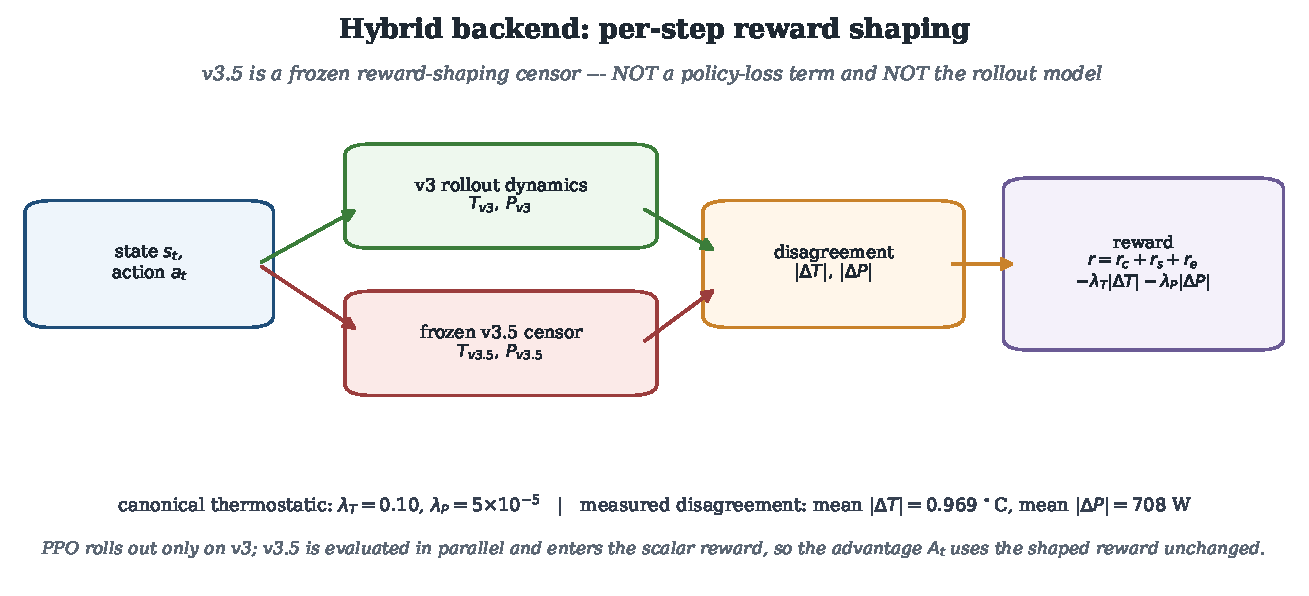
\includegraphics[width=0.90\linewidth]{fig_block2_reward_shaping.pdf}
  \caption{Hybrid reward-shaping mechanism. v3 supplies rollout dynamics; frozen v3.5 supplies a disagreement penalty on the same state-action transition.}
  \label{fig:hybrid_reward}

{\footnotesize\itshape Schematic; not derived from a dataset.}
\end{figure}

\subsection{Thermostatic PPO: direct-v3.5 failure and hybrid success (roadmap \S4--\S5)}

Table~\ref{tab:main_kpi} and Figure~\ref{fig:live_kpi} summarize the main Block 2 controller result. Pure v3 PPO is already usable ($m_s=0.073$ peak, $0.095$ typical). Direct v3.5 PPO fails catastrophically despite v3.5's superior Block 1 predictive fidelity: live violation reaches 77.1\% on peak and 82.4\% on typical, with RMSE above $4.3\,^\circ$C. The hybrid backend resolves the conflict: $m_s=0.087$ on peak and $0.041$ on typical, with violation below $5\%$ on both windows and lower energy than pure v3 on the peak window.

\begin{table}[pos={!ht}]
\centering
\caption{Canonical Block 2 live BOPTEST controller comparison on the targeted 14-day windows. Data sources for every row are catalogued in roadmap Section 11.1.}
\label{tab:main_kpi}
\small
\begin{tabular}{llrrrr}
\toprule
Policy/backend & Scenario & $m_s$ & Violation (\%) & RMSE$_T$ ($^\circ$C) & Energy (kWh) \\
\midrule
pure v3 PPO & peak & 0.073 & 1.49 & 0.869 & 322.2 \\
direct v3.5 PPO & peak & 1.046 & 77.08 & 4.320 & 556.2 \\
hybrid $\lambda_T=0.10$ & peak & 0.087 & 4.69 & 0.795 & 305.3 \\
pure v3 PPO & typical & 0.095 & 4.39 & 0.622 & 368.3 \\
direct v3.5 PPO & typical & 1.102 & 82.37 & 4.401 & 580.5 \\
hybrid $\lambda_T=0.10$ & typical & 0.041 & 2.38 & 0.633 & 352.8 \\
\bottomrule
\end{tabular}
\end{table}

\begin{figure}[pos={!ht}]
  \centering
  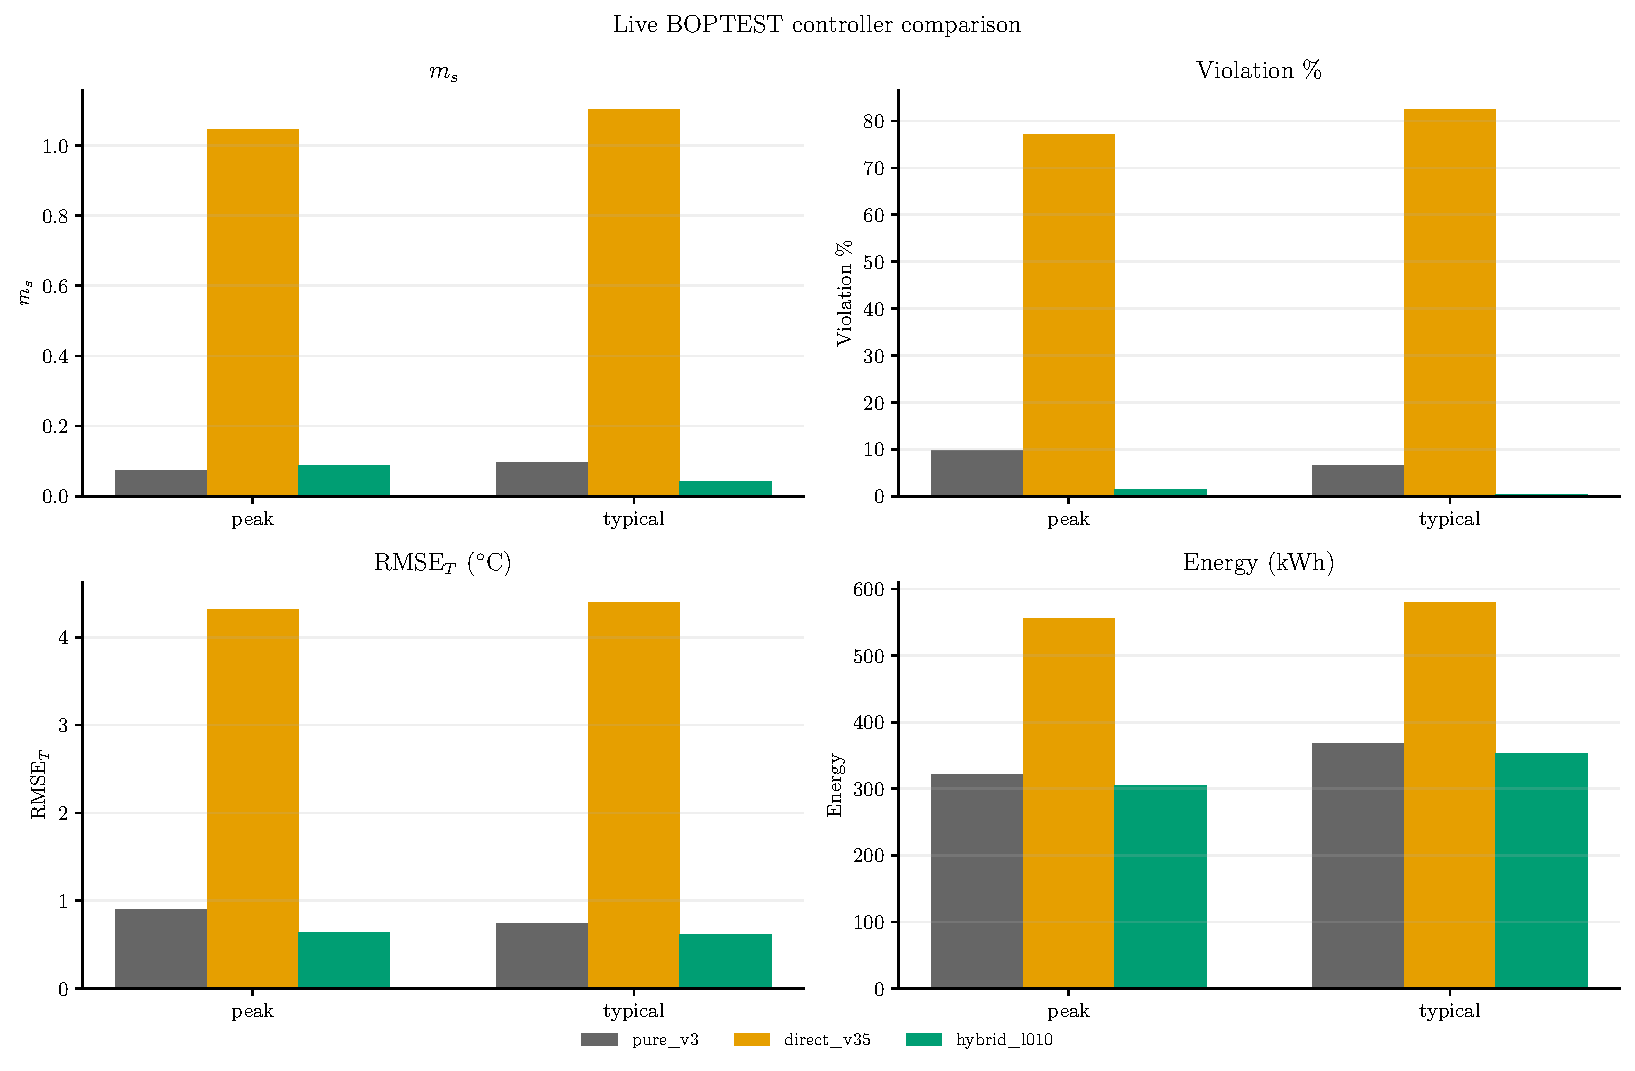
\includegraphics[width=0.96\linewidth]{final17_fig06_live_boptest_controller_comparison.pdf}
  \caption{Live BOPTEST KPI comparison for pure v3, direct v3.5, and hybrid PPO. Direct v3.5 is a negative control: higher predictive fidelity does not imply a useful RL training environment.}
  \label{fig:live_kpi}

{\footnotesize\itshape Data: \texttt{outputs/\allowbreak block2\_\allowbreak */\allowbreak summary.csv}}
\end{figure}

\paragraph{Reading $m_s$ step by step.} The decomposition $m_s=r_{\mathrm{time}}+r_{\mathrm{sev}}$ (Eq.~\ref{eq:ms}) exposes the failure structure directly (Figure~\ref{fig:ms_decomp}). Direct v3.5's peak $m_s=1.046$ is dominated by $r_{\mathrm{time}}\approx 0.77$ (out of band 77\% of the time) plus a large worst-case severity $r_{\mathrm{sev}}\approx 0.28$; the hybrid's peak $m_s=0.087$ is almost entirely a small $r_{\mathrm{sev}}$ with $r_{\mathrm{time}}<0.05$. The hybrid therefore does not merely lower the average error --- it removes the sustained band departures that dominate the direct-v3.5 score.

\begin{figure}[pos={!ht}]
  \centering
  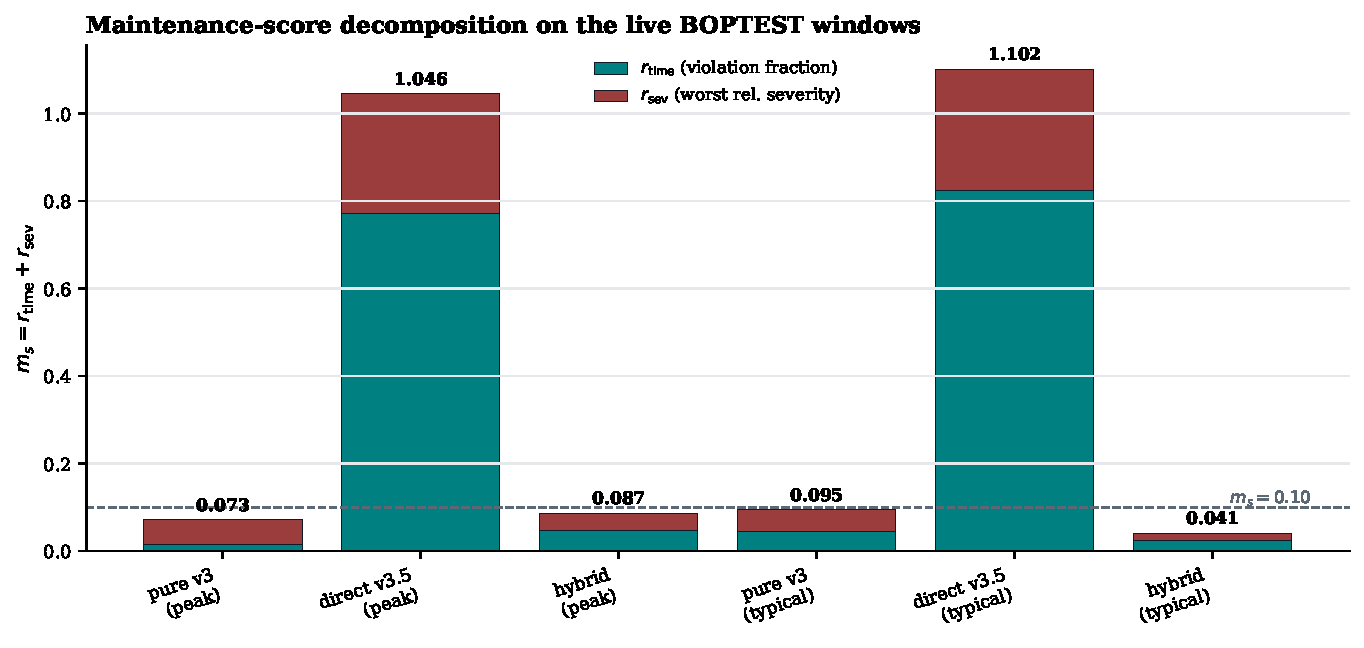
\includegraphics[width=0.82\linewidth]{fig_block2_ms_decomposition.pdf}
  \caption{Data-driven decomposition $m_s=r_{\mathrm{time}}+r_{\mathrm{sev}}$ on the live BOPTEST windows. Direct v3.5 fails through sustained violation ($r_{\mathrm{time}}$); pure v3 and the hybrid keep both terms small.}
  \label{fig:ms_decomp}

{\footnotesize\itshape Data: \texttt{outputs/\allowbreak block2\_\allowbreak */\allowbreak summary.csv}}
\end{figure}

The time-series and action diagnostics in Figures~\ref{fig:closed_loop_traces} and~\suppref{S8} explain the mechanism. Direct v3.5 learns a bang-bang-like control law that drives the live simulator outside the comfort band; in phase space it places extreme actions in temperature-error regimes the live building does not support. We note explicitly that this destabilization mechanism is \emph{hypothesized} (higher advantage-estimator variance under sharper surrogate predictions, and/or overfitting to sub-step physical structure unusable at the 15-min cadence) and is not directly measured here; discriminating the two is deferred to future work.

\begin{figure}[pos={!ht}]
  \centering
  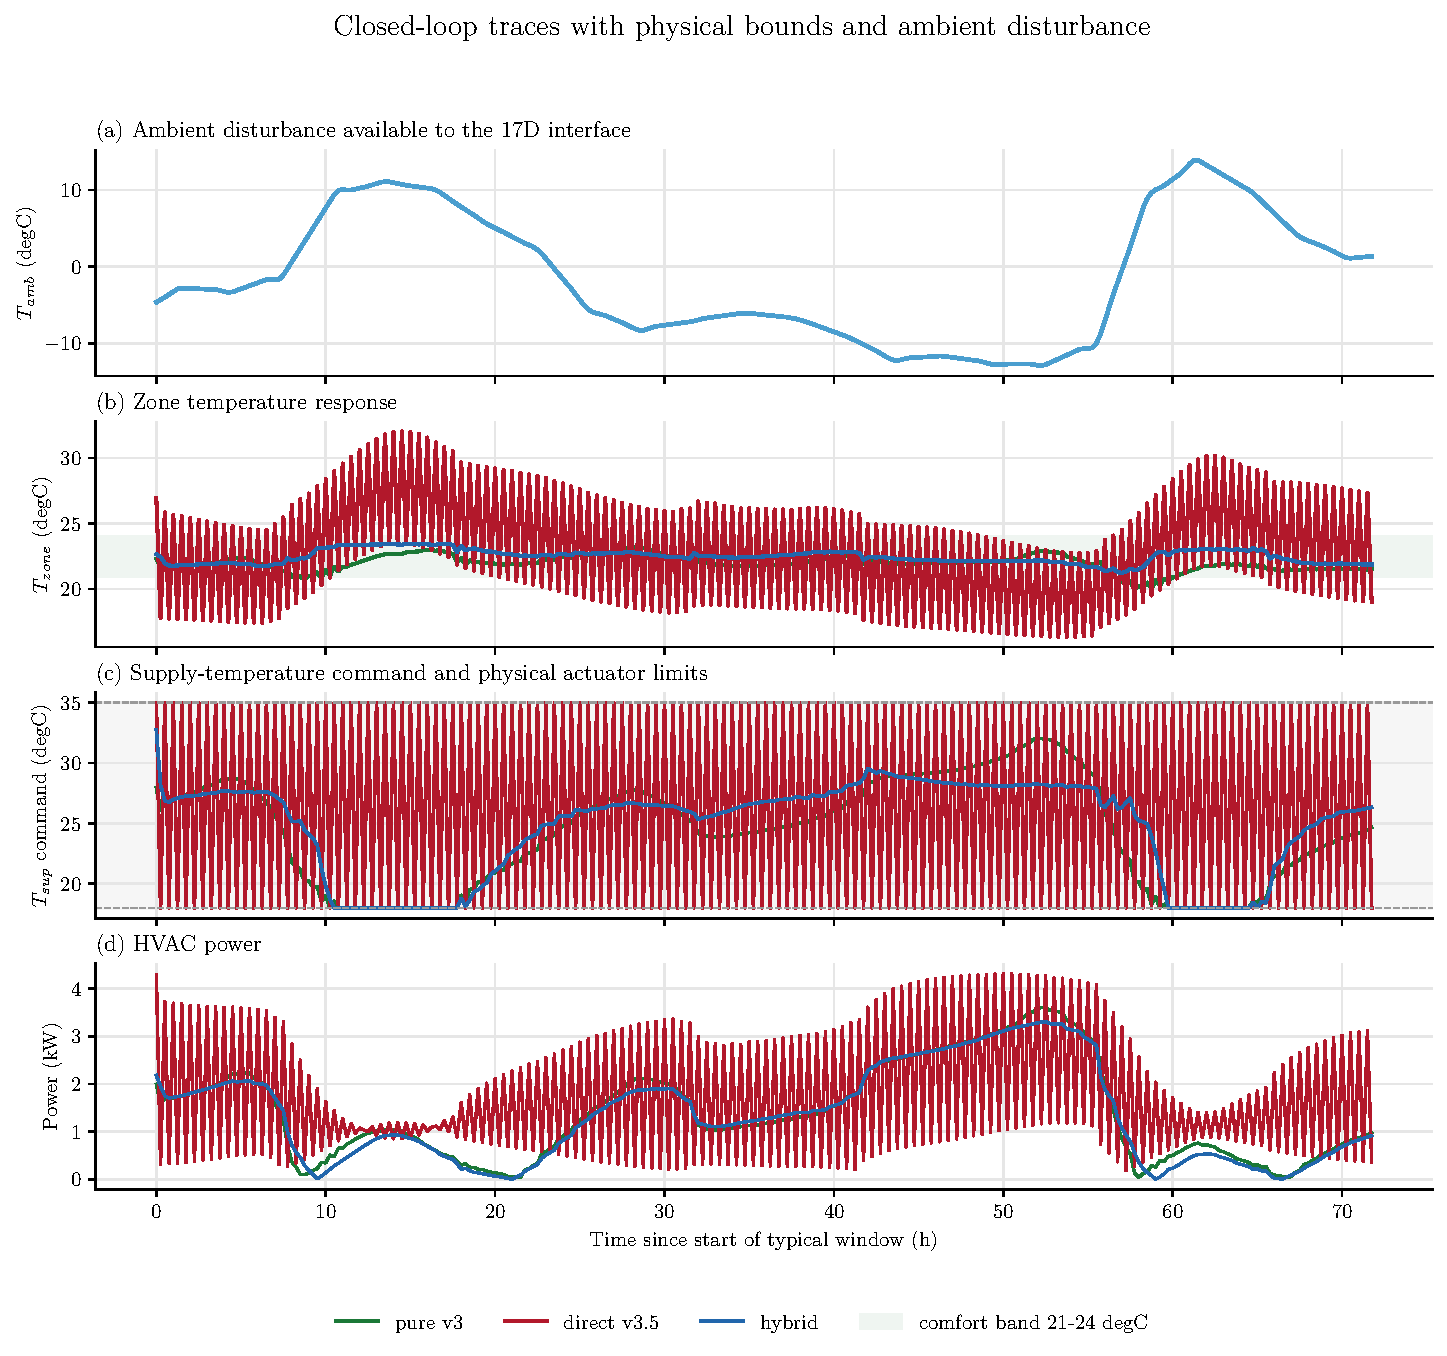
\includegraphics[width=0.96\linewidth]{block2_q1_polish_closed_loop_disturbance.pdf}
  \caption{Closed-loop BOPTEST traces with ambient disturbance, comfort band, and physical actuator limits.}
  \label{fig:closed_loop_traces}

{\footnotesize\itshape Data: \texttt{outputs/\allowbreak block2\_\allowbreak thermostatic\_\allowbreak hybrid\_\allowbreak v3\_\allowbreak v35\_\allowbreak l010/\allowbreak }}
\end{figure}



\paragraph{Hybrid $\lambda_T$ sweep and canonical selection (roadmap \S5).} The canonical hybrid operating point was selected by a thermostatic sweep over the temperature-disagreement weight $\lambda_T\in\{0.05,0.10,0.15\}$ at fixed $\lambda_P=5\times10^{-5}$ (Table~\suppref{S11}). The mid setting $\lambda_T=0.10$ (\texttt{hybrid\_l010}) is canonical: per the roadmap selection rule it retains the energy advantage over pure v3 while avoiding the stronger comfort degradation seen at the weaker ($0.05$) and stronger ($0.15$) censor settings. Only the canonical point's live-BOPTEST KPIs are retained as a frozen artifact; the bracketing points served selection only.



\subsection{Warm-start negative control (roadmap \S4.5)}

A second negative control tests whether v3.5 is useful as a policy \emph{initializer} rather than a reward-shaping censor. The benchmark (\texttt{run\_block2.py warmstart}) runs four steps: \emph{(1) pretrain} a thermostatic policy on the calibrated v3.5 surrogate; \emph{(2) scratch finetune} a thermostatic policy from random initialization directly on the live BOPTEST RTE; \emph{(3) warm-start finetune} a second policy on BOPTEST initialized from the v3.5-pretrained checkpoint of step~1; and \emph{(4) evaluate} both finetuned policies on the same BOPTEST windows and compare. The comparison is therefore internally controlled --- scratch and warm-start differ only in initialization. It does not help: warm-started policies are markedly worse than the scratch finetune (Table~\suppref{S12}), raising $m_s$ by roughly two to three times on both windows. The problem is the role assigned to the surrogate during early policy formation, not a lack of fine-tuning; v3.5 belongs in the reward as a censor, not in the weights as an initializer.



\begin{figure}[pos={!ht}]
  \centering
  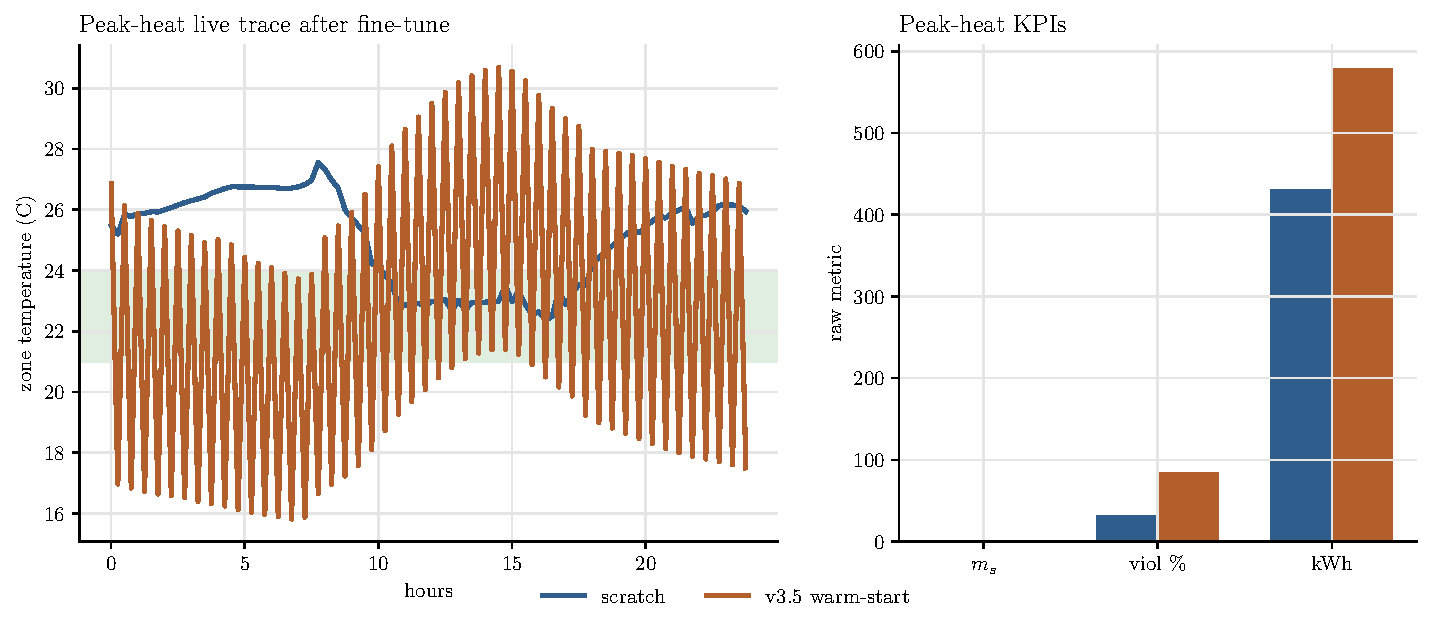
\includegraphics[width=0.82\linewidth]{block2_warmstart_negative_eval_kpis.pdf}
  \caption{Warm-start negative control. Pretraining on direct v3.5 and then fine-tuning on the hybrid backend is inferior to training the hybrid policy from scratch.}
  \label{fig:warmstart}

{\footnotesize\itshape Data: \texttt{outputs/\allowbreak block2\_\allowbreak thermostatic\_\allowbreak warmstart\_\allowbreak utility/\allowbreak comparison\_\allowbreak summary.csv}}
\end{figure}

\subsection{Transfer-gap diagnostics (roadmap \S5.5)}

This diagnostic (roadmap \S5.5) compares three controllers --- pure v3, hybrid $\lambda_T=0.10$, and direct v3.5 --- in three steps. \emph{Step 1}: a standalone direct-v3.5 thermostatic policy is trained on the calibrated v3.5 environment (the failure control; \texttt{thermostatic-train --variant v35\_direct}), separate from the warm-start checkpoint of the previous section because it answers a different question (zero-shot live transfer rather than warm-start utility). \emph{Step 2}: all three policies are run in closed loop on the live BOPTEST RTE for the two 14-day windows (\texttt{thermostatic-transfer --variant all}). \emph{Step 3}: for each policy we compute four transfer diagnostics (\texttt{thermostatic-diagnose}) --- the temperature tracking gap (live RMSE$_T$), the surrogate-vs-live maintenance-score mismatch
\begin{equation}
\begin{aligned}
  \Delta m_s &= m_s^{\mathrm{surrogate}} - m_s^{\mathrm{BOPTEST}}
  \qquad(\text{negative}\Rightarrow\text{surrogate optimistic}), \\[3pt]
  g_a &= \frac{1}{N}\sum_{t=1}^{N}\big\|\,a_t^{\mathrm{BOPTEST}}-a_t^{\mathrm{surrogate}}\,\big\|_{2} .
\end{aligned}
\label{eq:transfer_gap}
\end{equation}
the action-gap norm $g_a$, and the first divergence step (earliest 15-min step where surrogate and live trajectories separate beyond threshold), with the top driver feature attributed to the divergence.

Direct v3.5 has the largest transfer mismatch ($|\Delta m_s|\approx 0.9$--$1.0$, $g_a\approx 2.0$, live RMSE$_T>4.3\,^\circ$C), and its top divergence driver is $t_{\mathrm{zone}}$: its sharp temperature dynamics produce live actions unlike the surrogate rollout. Hybrid $\lambda_T=0.10$ has the smallest gap ($|\Delta m_s|\approx 0.02$) and, on the typical window, holds the BOPTEST-consistent action for 16 steps before drifting (Table~\ref{tab:transfer}). The action-gap norm is the most diagnostic column: $g_a=2.0$ for direct v3.5 means the policy sits at the opposite action bound from what BOPTEST would choose throughout the episode, i.e.\ a learned bang-bang exploit of the surrogate.

\begin{table}[pos={!ht}]
\centering
\caption{Transfer diagnostics across three backends. $\Delta m_s=$ surrogate $-$ live (negative $\Rightarrow$ surrogate optimistic); Temp gap is the live closed-loop RMSE$_T$ (data: roadmap Section 11.1).}
\label{tab:transfer}
\small
\begin{tabular}{llrrrrl}
\toprule
Variant & Scenario & Temp gap ($^\circ$C) & $\Delta m_s$ & Action gap & First div. & Top driver \\
\midrule
pure v3 & peak & 0.894 & -0.102 & 0.377 & 1 & p\_total\_norm \\
pure v3 & typical & 0.745 & -0.068 & 0.333 & 1 & p\_total\_norm \\
hybrid $\lambda_T=0.10$ & peak & 0.633 & -0.023 & 0.473 & 1 & p\_total\_norm \\
hybrid $\lambda_T=0.10$ & typical & 0.612 & -0.021 & 0.253 & 16 & p\_total\_norm \\
direct v3.5 & peak & 4.320 & -0.886 & 2.000 & 1 & t\_zone\_norm \\
direct v3.5 & typical & 4.401 & -1.014 & 2.014 & 1 & t\_zone\_norm \\
\bottomrule
\end{tabular}
\end{table}



\subsection{HDRL sensitivity: the hybrid weight is controller-family specific (roadmap \S6)}

HDRL here is a \emph{seasonal} hierarchy. A high-level seasonal selector routes control to one of two low-level PPO setpoint specialists --- a winter agent (trained 5M steps on cold-season day ranges with cold-biased comfort shaping) and a summer agent (7M steps on warm-season ranges) --- each acting on the same 17D observation and supply-temperature action. Formally the controller is $\pi(a_t\mid s_t)=\pi_{k(t)}(a_t\mid s_t)$ with the high-level gate $k(t)\in\{\text{winter},\text{summer}\}$ chosen by season; the hierarchy supplies regime-aware temporal abstraction, so each low-level specialist solves a narrower, better-conditioned control problem than a single global policy (Figure~\ref{fig:hdrl_arch}).

\begin{figure}[pos={!ht}]
  \centering
  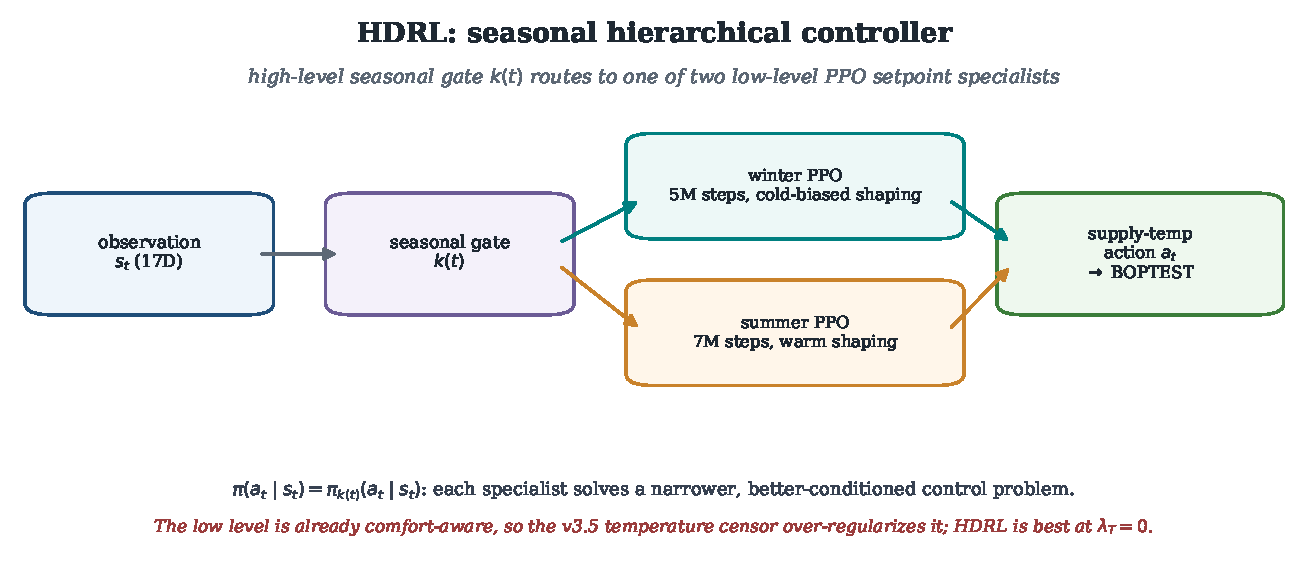
\includegraphics[width=0.96\linewidth]{fig_block2_hdrl_architecture.pdf}
  \caption{HDRL architecture: a high-level seasonal gate $k(t)$ routes the 17D observation to one of two low-level PPO setpoint specialists (winter / summer). Because the low level is already comfort-aware, the v3.5 temperature censor over-regularizes it.}
  \label{fig:hdrl_arch}

{\footnotesize\itshape Schematic; not derived from a dataset.}
\end{figure}

The HDRL experiment asks whether the thermostatic hybrid setting $\lambda_T=0.10$ transfers to this hierarchical controller. It does not (Table~\ref{tab:hdrl}). The mechanism is over-regularization: because each seasonal specialist already encodes comfort-aware structure (season-tuned shaping plus the high-level gate), the additional v3.5 temperature-disagreement censor constrains an already comfort-aware low-level loop, biasing it toward conservative under-heating; performance therefore degrades monotonically with $\lambda_T$, and the correct transfer keeps only the power channel ($\lambda_T=0$). HDRL performs best at $\lambda_T=0.00$ on both windows and degrades monotonically as temperature-disagreement regularization is increased. This shows the correct physical-censor strength depends on the controller family and its action decomposition, not on a universal weight.

\begin{table}[pos={!ht}]
\centering
\caption{HDRL sweep over $\lambda_T$ on the targeted windows; best is $\lambda_T=0$, and performance degrades monotonically as the temperature censor strengthens (data: roadmap Section 11.1).}
\label{tab:hdrl}
\small
\begin{tabular}{llrrrr}
\toprule
$\lambda_T$ & Scenario & $m_s$ & Violation (\%) & RMSE$_T$ ($^\circ$C) & Energy (kWh) \\
\midrule
0.00 & peak & 0.180 & 6.10 & 0.751 & 329.6 \\
0.03 & peak & 0.307 & 11.90 & 0.993 & 311.5 \\
0.05 & peak & 0.418 & 20.98 & 1.303 & 298.1 \\
0.10 & peak & 0.440 & 22.99 & 1.343 & 300.4 \\
0.00 & typical & 0.234 & 3.12 & 0.691 & 385.1 \\
0.03 & typical & 0.296 & 9.38 & 0.959 & 369.6 \\
0.05 & typical & 0.512 & 27.38 & 1.491 & 354.5 \\
0.10 & typical & 0.511 & 30.65 & 1.455 & 357.1 \\
\bottomrule
\end{tabular}
\end{table}

\paragraph{Engineering reading.} As $\lambda_T$ rises, energy falls slightly (the censor biases the low-level loop toward conservative under-heating, e.g. $329.6\to300.4$ kWh on peak) but comfort collapses --- peak violation roughly quadruples ($6.1\%\to23.0\%$) and RMSE$_T$ nearly doubles. HDRL already supplies comfort-aware temporal abstraction through its scheduler, so an additional temperature-disagreement censor is redundant and over-constrains the setpoint controller; the correct transfer of the Block 1 recipe to HDRL keeps only the power channel ($\lambda_T=0$, $\lambda_P=5\times10^{-5}$).

\begin{figure}[pos={!ht}]
  \centering
  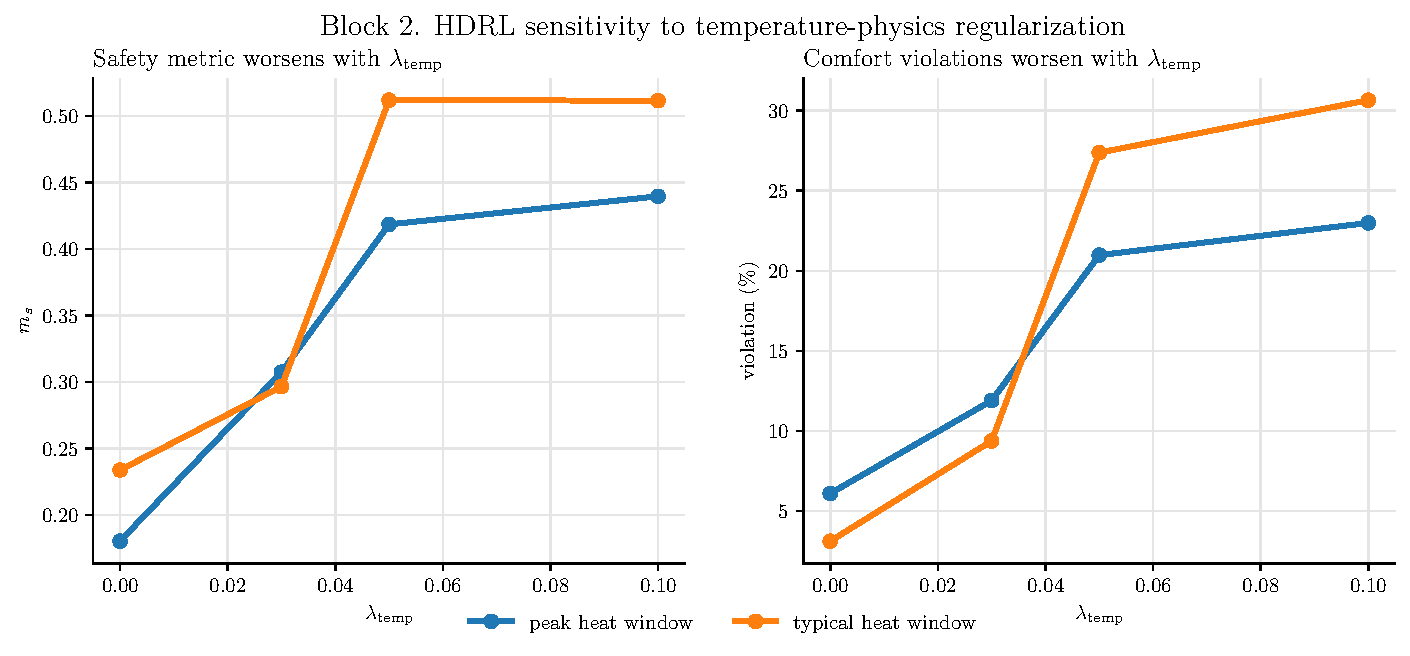
\includegraphics[width=0.88\linewidth]{block2_hdrl_lambda_sweep_sensitivity.pdf}
  \caption{HDRL $\lambda_T$ sensitivity. The thermostatic regularization weight does not transfer; the best HDRL policy uses no temperature-disagreement term.}
  \label{fig:hdrl_sweep}

{\footnotesize\itshape Data: \texttt{reports/\allowbreak block2\_\allowbreak hdrl\_\allowbreak lambda\_\allowbreak sweep\_\allowbreak summary.csv}}
\end{figure}

\subsection{MORL observation ablation: 5D failure to 17D success (roadmap \S6.5--\S7)}

MORL uses a four-stage pipeline that differs from the single-stage PPO families (roadmap Section 7): (1) a 2M-step surrogate \emph{pretrain} on the 17D hybrid backend with canonical $(w_c,w_e,w_s)=(0.80,0.20,0.00)$; (2) an \emph{ERAM} weight-adaptation stage (20 iterations of 100k steps from initial weights $0.34/0.33/0.33$, weight-update temperature $\tau_w=0.35$); (3) a 100k-step \emph{finetune} on the live BOPTEST RTE at learning rate $10^{-4}$ with $\pm3$-day episode-start jitter; and (4) a 12-month \emph{yearly evaluation}. MORL is the only family with a live-BOPTEST finetune; the thermostatic/HDRL families are evaluated zero-shot after surrogate-only training, which is a strictly harder transfer (Figure~\suppref{S10}).



MORL initially failed with a 5D observation (zone temperature, ambient, hour, day, occupancy). Under the current code path, a reconstructed 5D rerun obtains RMSE$_T=2.721\,^\circ$C, violation $37.8\%$, and $m_s=0.680$; the originally frozen 5D artifact was even worse (RMSE$_T=4.96\,^\circ$C, $m_s=1.046$) and is retained only as an audit artifact. Replacing the observation with the 17D TSup-style vector recovers a usable policy: RMSE$_T=0.720\,^\circ$C, violation $4.9\%$, $m_s=0.099$ (Table~\ref{tab:morl5d17d}). The dominant MORL bottleneck was the observation geometry, not the reward scalarization alone.

\begin{table}[pos={!ht}]
\centering
\caption{MORL observation-interface ablation. The backend is hybrid in both cases; only the observation interface changes. The current-code reconstructed 5D rerun is the reproducible main-paper evidence (roadmap Section 11.1).}
\label{tab:morl5d17d}
\small
\begin{tabular}{lrrrr}
\toprule
Variant & Obs dim & RMSE$_T$ ($^\circ$C) & Violation (\%) & $m_s$ \\
\midrule
MORL 5D (current-code rerun) & 5 & 2.721 & 37.8 & 0.680 \\
MORL 17D power-only (canonical) & 17 & 0.720 & 4.9 & 0.099 \\
\bottomrule
\end{tabular}
\end{table}

\begin{figure}[pos={!ht}]
  \centering
  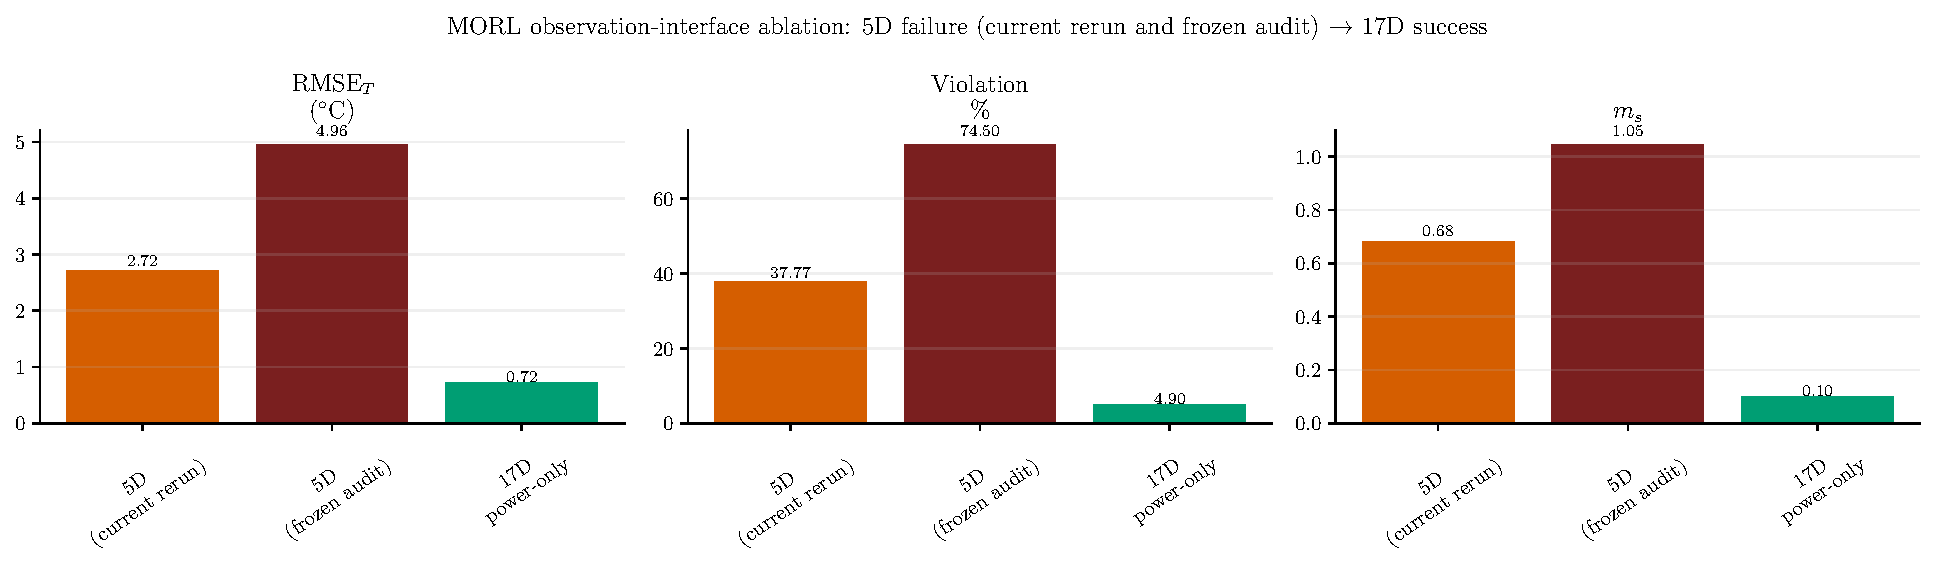
\includegraphics[width=0.84\linewidth]{final17_fig09_morl_5d_failure_17d_success.pdf}
  \caption{MORL 5D failure and 17D recovery. The observation interface, not only the scalarized reward, determines whether MORL is viable.}
  \label{fig:morl5d17d}

{\footnotesize\itshape Data: \texttt{reports/\allowbreak block2\_\allowbreak morl\_\allowbreak 5d\_\allowbreak reconstructed\_\allowbreak comparison.csv}}
\end{figure}

\paragraph{Power-only backend and claim discipline (roadmap \S7, \S9, \S13).} MORL inherits the controller-family lesson of the HDRL sweep: it runs on the \emph{power-only} hybrid backend ($\lambda_T=0$, $\lambda_P=5\times10^{-5}$), because temperature-disagreement censoring hurts non-thermostatic families. The MORL claim is deliberately narrow and audit-protected. Before the seed expansion, commit \texttt{93df9b3} froze the canonical plan and the seed-45/46 falsification predictions; after $N=5$, commit \texttt{62dc859} appended the observed variance without rewriting the pre-specification, and a replay test confirmed bit-identical BOPTEST trajectories for a fixed checkpoint (so the spread is training stochasticity, not simulator noise). The defensible reading is therefore: under the fixed 17D power-only backend, MORL is substantially stronger than the reconstructed 5D interface and yields a usable comfort--energy Pareto structure, but the $N=5$ canonical variance (CV $0.42$--$0.61$) is too high for a deployment-stability claim --- the single-seed canonical is the best of five, not the median.

\subsection{MORL Pareto front and N=5 seed variance (roadmap \S8--\S9)}

The MORL Pareto sweep varies comfort/energy weights with safety weight zero (Table~\ref{tab:morl_pareto_seed}). Energy-only control collapses comfort ($m_s=1.588$, violation $86.8\%$); comfort-leaning settings are far more stable. The single-seed (seed 42) Pareto points are reported separately from the $N=5$ canonical extensions, because the seed analysis is the central audit result: the neutral 50/50 canonical has $m_s=0.187\pm0.078$ (CV $0.42$, 95\% $t$-CI $[0.090,0.284]$) and the practical 75/25 canonical has $m_s=0.139\pm0.085$ (CV $0.61$, 95\% $t$-CI $[0.033,0.245]$). Seed 46 is an outlier in both groups (Table~\suppref{S13}). Because the replay audit produced bit-identical BOPTEST trajectories for a fixed policy, this variance is attributed to PPO/ERAM training stochasticity, not simulator noise. The single-seed canonical ($m_s\approx0.10$) is therefore the \emph{best} of five, not the median.

\begin{table}[pos={!ht}]
\centering
\caption{MORL Pareto (seed 42) and N=5 canonical seed analysis (data: roadmap Section 11.1).}
\label{tab:morl_pareto_seed}
\small
\begin{tabular}{lrrll}
\toprule
Preference / statistic & RMSE$_T$ ($^\circ$C) & Violation (\%) & $m_s$ & Interpretation \\
\midrule
0/100 (seed 42) & 8.359 & 86.76 & 1.588 & energy-only collapse \\
25/75 (seed 42) & 0.912 & 11.39 & 0.173 & energy-weighted usable \\
50/50 (N=5 mean$\pm$std) & 0.893$\pm$0.081 & 13.01$\pm$6.62 & 0.187$\pm$0.078 & neutral, CV=0.42 \\
75/25 (N=5 mean$\pm$std) & 0.799$\pm$0.100 & 9.23$\pm$6.67 & 0.139$\pm$0.085 & practical, CV=0.61 \\
100/0 (seed 42) & 0.631 & 1.49 & 0.032 & best seed-42 comfort \\
\bottomrule
\end{tabular}
\end{table}

\paragraph{Engineering reading.} The front is strongly asymmetric. Energy-only control (0/100) collapses to a degenerate non-heating policy ($86.8\%$ violation, $m_s=1.588$): minimizing energy simply means not heating. Comfort-only (100/0) is the best single-seed $m_s$ but the most energy-hungry, and the practical 75/25 point recovers near-comfort-only comfort at lower energy --- the recommended deployment compromise. The crucial caveat is the seed dimension: the single-seed front overstates reliability, because the $N=5$ extension turns both canonicals into wide distributions (CV $0.42$--$0.61$), so the Pareto curve should be read as a best-seed envelope, not a deployment guarantee.

\begin{figure}[pos={!ht}]
  \centering
  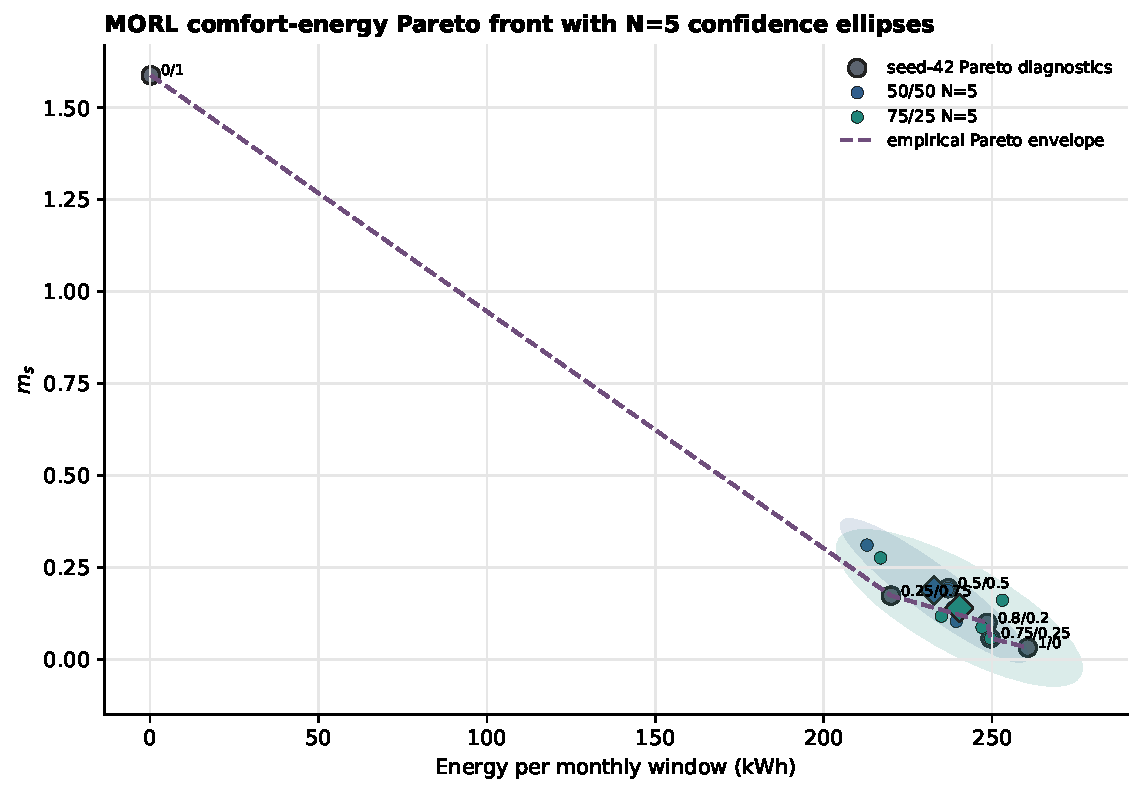
\includegraphics[width=0.86\linewidth]{block2_q1_polish_morl_pareto_ellipses.pdf}
  \caption{MORL comfort--energy Pareto front with N=5 confidence ellipses for the two canonical points. Non-canonical points are seed-42 only.}
  \label{fig:morl_pareto}

{\footnotesize\itshape Data: \texttt{reports/\allowbreak morl\_\allowbreak pareto\_\allowbreak front\_\allowbreak table.csv}}
\end{figure}



\subsection{Seasonal variance falsification (roadmap \S9; audit \S13)}

At $N=3$, the practical canonical appeared to show near-deterministic winter behavior and a seasonal inversion relative to the neutral canonical, motivating a pre-specified falsification test before seeds 45 and 46 were trained. The direction-specific predictions (February winter $\sigma(m_s)<0.005$; June summer $\sigma(m_s)>0.05$; winter neutral/practical variance ratio $>20$) failed at $N=5$: February practical $\sigma(m_s)$ rose to order $0.17$ and the winter variance ratio collapsed to order one. This is a success of the pre-specification protocol (audit anchors \texttt{93df9b3} pre-specification, \texttt{62dc859} post-N=5 falsification), not a project failure. The honest, narrower conclusion: MORL is promising in mean performance, especially at comfort-leaning preferences, but is \emph{not} deployment-stable without explicit stabilization (validation-based checkpoint selection, early stopping, or ensemble selection), which is left as future work because the canonical protocol fixes final-epoch evaluation.





\subsection{PI reference and synthesis (roadmap \S10--\S11)}

The BOPTEST built-in PI controller is a reproducible reference, not a tuned strong baseline. On the 12-month yearly evaluation it is comfort-poor but energy-frugal: mean RMSE$_T=3.40\,^\circ$C, mean violation $63.6\%$, mean monthly energy $104.1$ kWh, mean $m_s=0.910$. All Block 2 RL/MORL agents reach $m_s$ well below PI's $0.910$, dominating it on comfort at comparable or lower energy after accounting for the comfort/energy trade-off.

Table~\ref{tab:ms_decomp} consolidates the maintenance-score decomposition across every controller family. It makes the cross-family pattern explicit: usable controllers (pure v3, hybrid, MORL 17D) keep both $r_{\mathrm{time}}$ and $r_{\mathrm{sev}}$ small, whereas the failures (direct v3.5, PI) carry a large $r_{\mathrm{time}}$ --- they spend a large fraction of the horizon outside the band. PI is the mirror image of direct v3.5: both have $r_{\mathrm{time}}$ near or above $0.6$, but PI fails by chronic under-heating while direct v3.5 fails by saturated overshoot.

\begin{table}[pos={!ht}]
\centering
\caption{Cross-controller maintenance-score decomposition $m_s = r_{\mathrm{time}} + r_{\mathrm{sev}}$ (Eq.~\ref{eq:ms}). $r_{\mathrm{time}}$ = fraction of steps outside the band; $r_{\mathrm{sev}}$ = worst relative band exceedance. Thermostatic/HDRL rows are 14-day windows; MORL/PI rows are 12-month yearly means.}
\label{tab:ms_decomp}
\small
\begin{tabular}{lrrr}
\toprule
Controller (window/eval) & $m_s$ & $r_{\mathrm{time}}$ & $r_{\mathrm{sev}}$ \\
\midrule
pure v3 (peak) & 0.073 & 0.015 & 0.058 \\
direct v3.5 (peak) & 1.046 & 0.771 & 0.276 \\
hybrid $\lambda_T{=}0.10$ (peak) & 0.087 & 0.047 & 0.040 \\
HDRL $\lambda_T{=}0$ (peak) & 0.180 & 0.061 & 0.119 \\
pure v3 (typical) & 0.095 & 0.044 & 0.051 \\
direct v3.5 (typical) & 1.102 & 0.824 & 0.278 \\
hybrid $\lambda_T{=}0.10$ (typical) & 0.041 & 0.024 & 0.017 \\
HDRL $\lambda_T{=}0$ (typical) & 0.234 & 0.031 & 0.202 \\
MORL 50/50 (yearly, N=5) & 0.187 & 0.130 & 0.057 \\
MORL 75/25 (yearly, N=5) & 0.139 & 0.092 & 0.047 \\
PI (yearly) & 0.910 & 0.636 & 0.274 \\
\bottomrule
\end{tabular}
\end{table}

Block 2 establishes four controller-side claims. First, predictive fidelity and RL training utility are not equivalent: direct v3.5 is the more accurate twin yet fails as a rollout environment (live violation $>77\%$). Second, role separation works --- v3 provides smooth rollout dynamics while frozen v3.5 acts as a physical censor through disagreement shaping --- giving the canonical hybrid ($m_s=0.087$ peak, $0.041$ typical). Third, the censor strength is controller-family specific: HDRL rejects $\lambda_T=0.10$ and is best at $\lambda_T=0$. Fourth, MORL is viable only with the 17D interface, and its N=5 analysis reveals high seed variance and falsifies the N=3 seasonal-inversion mechanism. The engineering implication is that hybrid surrogate RL is a role-allocation problem --- rollout smoothness, physical censoring, observation geometry, controller family, and seed stabilization are separate design axes. This is the bridge to Block 3, where the fixed \texttt{bestest\_air} recipe is transferred to the hydronic BOPTEST family.

% Auto-generated by docs/build_integrated_paper.py -- do not edit by hand.
% Standalone scaffolding (preamble, nomenclature, limitations, conclusion,
% \setcounter) stripped for \input into the combined manuscript.
\section{Results III: Transferability Hypothesis}
\label{sec:results3-transfer}

\subsection{Block 3 objective and evidence boundary}

Blocks 1 and 2 established the source-case recipe on BOPTEST \texttt{bestest\_air}: a v3 rollout surrogate supplies smooth control-oriented dynamics, a calibrated v3.5 RC--NeuralODE supplies a frozen physical disagreement censor, and the thermostatic PPO policy trained on the resulting hybrid backend is the strongest verified controller on the targeted windows. Block 3 asks a narrower, more falsifiable question: does this fixed source-case recipe transfer to related BOPTEST hydronic-family testcases?

The claim boundary is deliberately limited. Block 3 does not claim universal building generalization, cross-climate generalization, or transfer to arbitrary HVAC topologies. It evaluates transfer to three pre-selected single-zone hydronic-family cases under documented actuator adapters and pre-specified recalibration regimes, with controller fine-tuning on the target testcase explicitly excluded. That exclusion is methodologically central: it separates \emph{controller} transfer from \emph{surrogate-recalibration} transfer, so the evidence is reported component-wise.

\paragraph{Roadmap boundary and executed path.}
Block 3 (\texttt{roadmap.md} Sections 14--15) was opened only after the Block 1/2 article state was committed, and runs strictly as:
\begin{enumerate}
  \item pre-specify the testcase/regime/hypothesis manifest before any non-\texttt{bestest\_air} run (\S14);
  \item for each testcase, smoke-test the actuator adapter, run the PI baseline, and run mode=none frozen-controller transfer (\S15.1--15.2);
  \item collect target telemetry and run partial (Stage C) and full (Stage A/B/C) surrogate recalibration (\S15.2);
  \item aggregate the transfer matrix and close the pre-specified hypotheses (\S15.3--15.5).
\end{enumerate}
Artifact provenance and rebuild commands for every table and figure are catalogued in roadmap Section 15.



\subsection{Pre-specification and audit anchors}

Block 3 is pre-specified through \texttt{configs/block3\_testcase\_manifest.yaml}. The initial manifest commit (\texttt{1861e48}) was made before any non-\texttt{bestest\_air} BOPTEST run; the pre-specification block is bit-identical between that commit and the close commit, with only result appendices added. The audit anchors are: \texttt{1861e48} (pre-specification manifest), \texttt{2f9d596} (record pre-specification SHA), \texttt{eb7091e} / \texttt{46fbaa9} / \texttt{645626e} (the three actuator adapters and the stretch-testcase predictions), \texttt{7ada793} (close SHA), and \texttt{cb7025f} (component-level interpretation). Because the hypothesis definitions were frozen before the runs, every number below was predictable but not predicted.

\subsection{Testcases, actuator adapters, and recalibration regimes}

The three target testcases span an increasing difficulty ladder relative to \texttt{bestest\_air}; all are single-zone or single-zone-like, heating-capable, and structurally non-identical to the source case.



The adapter maps the frozen source policy output to the target actuator interface:
\begin{equation}
  u^{\mathrm{target}}_t = \mathcal{A}_{k}\!\left(T^{\mathrm{sup}}_t,\, y_t\right),
  \qquad
  T^{\mathrm{sup}}_t = 18 + \tfrac{a_t+1}{2}(35-18),
  \label{eq:adapter}
\end{equation}
where $\mathcal{A}_{k}$ is the pre-specified adapter for testcase $k$, $a_t\in[-1,1]$ is the frozen policy output, and $y_t$ are available BOPTEST measurements used by rule-based adapter logic. Adapter smoke tests verify that low/high overrides produce directionally valid heating before any yearly run. Figure~\suppref{S14} shows the adapter-mediated transfer: one frozen controller drives three different actuator interfaces through the per-testcase adapters, with per-testcase controller verdicts. The recalibration regimes (Table~\suppref{S16}) keep the controller frozen and vary only how much of the surrogate adapts.



Concretely, each adapter first maps the policy command to a normalized heat-intensity $h=\mathrm{clip}\!\big((T^{\mathrm{sup}}_t-18)/17,\,0,\,1\big)$ and then drives the testcase's pre-specified BOPTEST override inputs (Table~\suppref{S15}). The mappings were finalized and committed before any control run (audit anchors \texttt{eb7091e} / \texttt{46fbaa9} / \texttt{645626e}), so the actuator interface cannot be tuned post hoc.





\subsection{Testcase architecture and physical processes}

The three targets differ in heat source, distribution path, and actuator set, but share the same single-zone energy balance (Figure~\ref{fig:topology}). For a hydronic zone the governing first-order balance is
\begin{equation}
  C_{\mathrm{zon}}\frac{dT_{\mathrm{zon}}}{dt} = \dot{Q}_{\mathrm{hyd}}(u_t) + \frac{T_{\mathrm{amb}}-T_{\mathrm{zon}}}{R_{\mathrm{env}}} + \dot{Q}_{\mathrm{gain}},
  \label{eq:hydronic_balance}
\end{equation}
where $\dot{Q}_{\mathrm{hyd}}$ is the delivered hydronic heat (whose actuation path --- heat pump, boiler/radiator, or district valve --- changes per testcase), $R_{\mathrm{env}}$ the envelope resistance, and $\dot{Q}_{\mathrm{gain}}$ the internal/solar gains. Transfer changes the \emph{delivery path} $\dot{Q}_{\mathrm{hyd}}$ and the actuator interface, but $C_{\mathrm{zon}}$ is the shared physical invariant that Stage~B re-identifies --- which is why its re-identified value transfers (Section~\ref{ssec:czon}).

\begin{figure}[H]
  \centering
  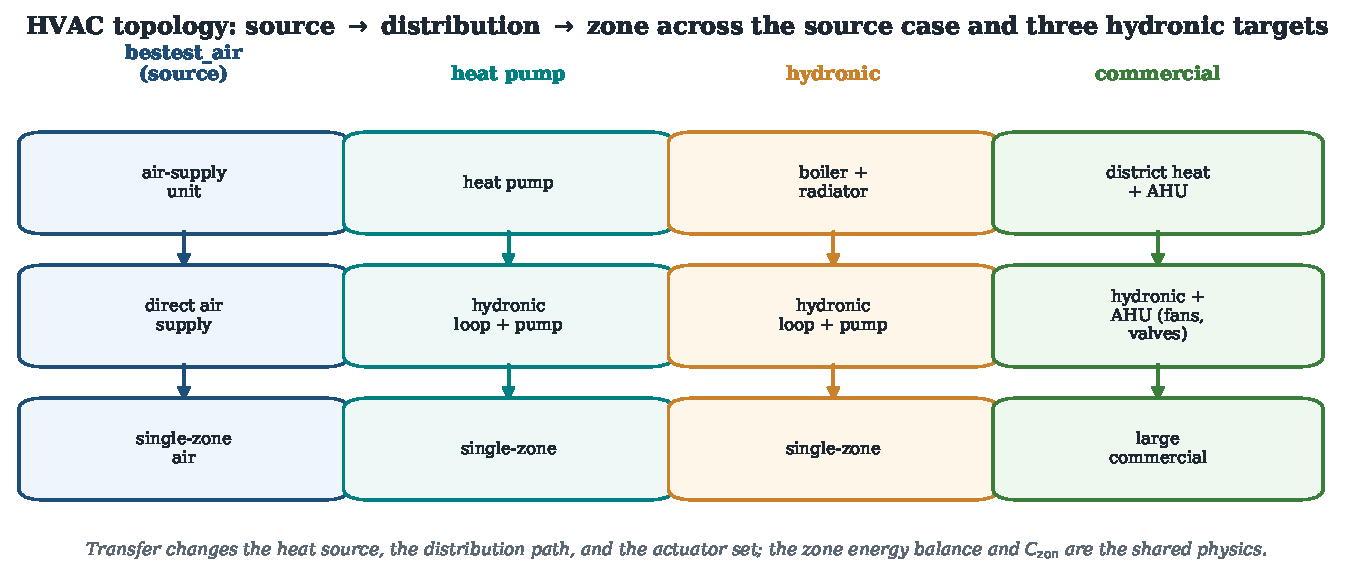
\includegraphics[width=0.97\linewidth]{fig_block3_topology.pdf}
  \caption{Comparative HVAC topology of the source case and the three hydronic targets (source $\to$ distribution $\to$ zone). Transfer changes the heat source, distribution path, and actuator set, while the zone energy balance \eqref{eq:hydronic_balance} and $C_{\mathrm{zon}}$ are shared.}
  \label{fig:topology}

{\footnotesize\itshape Schematic; not derived from a dataset.}
\end{figure}

Table~\ref{tab:physics} summarizes the architecture and the identified physics. The equivalent thermal mass $C_{\mathrm{zon}}/c_{p,\mathrm{air}}$ (with $c_{p,\mathrm{air}}=1005$~J\,kg$^{-1}$K$^{-1}$) is roughly $2\times$ the \texttt{bestest\_air} value for every hydronic case, consistent with the added water-loop and surface thermal mass. The mean delivered power exposes the operating regime: it is of order $10^3$~W for the residential cases (envelope-conduction / slow-hydronic dominated) but two orders of magnitude larger for the commercial case (roughly $28\times$), because that zone is ventilation/AHU-dominated. This ventilation dominance is the physical reason the commercial controller passes the comfort threshold yet overshoots energy by $+35.3\%$; it also makes a conduction-only time constant ill-defined from total power for that case.

\begin{table}[H]
\centering
\small
\caption{Testcase architecture and identified physics. $C_{\mathrm{zon}}$ in $10^5$~J/K; equivalent mass $=C_{\mathrm{zon}}/c_{p,\mathrm{air}}$; mean delivered power from the Stage-C telemetry.}
\label{tab:physics}
\begin{tabularx}{\linewidth}{l l r r r >{\raggedright\arraybackslash}X}
\toprule
Testcase & Heat source & $C_{\mathrm{zon}}$ & eq.\ mass (kg) & mean power (W) & Thermal regime \\
\midrule
\texttt{bestest\_air} (source) & air supply & 4.413 & 439 & --- & reference \\
\midrule
hydronic heat pump & heat pump & 8.348 & 831 & 2,778 & conduction-dominated \\
hydronic (boiler) & boiler/radiator & 8.623 & 858 & 679 & slow hydronic \\
commercial hydronic & district + AHU & 8.426 & 838 & 76,860 & ventilation/AHU-dominated \\
\bottomrule
\end{tabularx}
\end{table}

\subsection{Engineering metrics and pass/fail rules}

The controller-side pass threshold is normalized by each testcase's built-in PI baseline, and energy is reported on a separate axis:
\begin{equation}
  \tau_k = 1.25\,m_{s,\mathrm{PI},k},
  \qquad
  \mathrm{PASS}^{\mathrm{ctrl}}_k = \mathbf{1}\!\left[\,m_{s,\mathrm{RL},k} \le \tau_k\,\right],
  \qquad
  \Delta E_k = 100\,\frac{E_{\mathrm{RL},k}-E_{\mathrm{PI},k}}{E_{\mathrm{PI},k}}.
  \label{eq:threshold}
\end{equation}
The threshold value $1.25$ was pre-specified, not chosen post hoc. Surrogate-side transfer is measured by the relative rollout-RMSE improvement after full Stage A/B/C recalibration, and the physical transfer diagnostic is the re-identified capacitance ratio:
\begin{equation}
  G^{\mathrm{RMSE}}_k = 100\,\frac{\mathrm{RMSE}^{\mathrm{raw}}_{T,k}-\mathrm{RMSE}^{\mathrm{full}}_{T,k}}{\mathrm{RMSE}^{\mathrm{raw}}_{T,k}},
  \qquad
  \rho_{C,k} = C^{(k)}_{\mathrm{zon}} \big/ C^{\mathrm{air}}_{\mathrm{zon}},
  \quad C^{\mathrm{air}}_{\mathrm{zon}} = 4.413\times10^5~\mathrm{J/K}.
  \label{eq:gain_ratio}
\end{equation}
Two-axis reporting ($m_s$ threshold and $\Delta E$) is necessary because the commercial testcase passes the $m_s$ bound while consuming substantially more energy than PI.

\subsection{Headline transfer matrix}

Table~\ref{tab:transfer_matrix} is the compact evidence summary and contains two distinct stories. The surrogate component transfers strongly: full Stage A/B/C improves RMSE by $60.2$--$87.8\%$ on all three target testcases. The frozen controller does not transfer uniformly: the two residential hydronic cases fail the pre-specified $1.25\times$ PI threshold, while the commercial stretch case passes the threshold but pays a $+35.3\%$ energy penalty.

\begin{table}[H]
\centering
\scriptsize
\caption{Block 3 transfer matrix. Threshold $=1.25\,m_{s,\mathrm{PI}}$ per testcase; data sources in roadmap Section 15. $^\dagger$ threshold PASS, not deployment-ready (see $\Delta E$).}
\label{tab:transfer_matrix}
\begin{tabular}{lrrrlrrrrr}
\toprule
Testcase & $m_s^{\mathrm{RL}}$ & $m_s^{\mathrm{PI}}$ & $\tau_k$ & Ctrl. & $\Delta E$\% & Raw RMSE & Full RMSE & Gain\% & $\rho_C$ \\
\midrule
hydronic heat pump & 0.665 & 0.464 & 0.579 & FAIL & -7.3 & 1.421 & 0.565 & 60.2 & 1.892 \\
hydronic (boiler) & 0.976 & 0.750 & 0.938 & FAIL & -5.8 & 2.666 & 0.335 & 87.4 & 1.954 \\
commercial hydronic & 0.431 & 0.628 & 0.785 & PASS$^\dagger$ & 35.3 & 1.952 & 0.238 & 87.8 & 1.909 \\
\bottomrule
\end{tabular}
\end{table}

\begin{figure}[H]
  \centering
  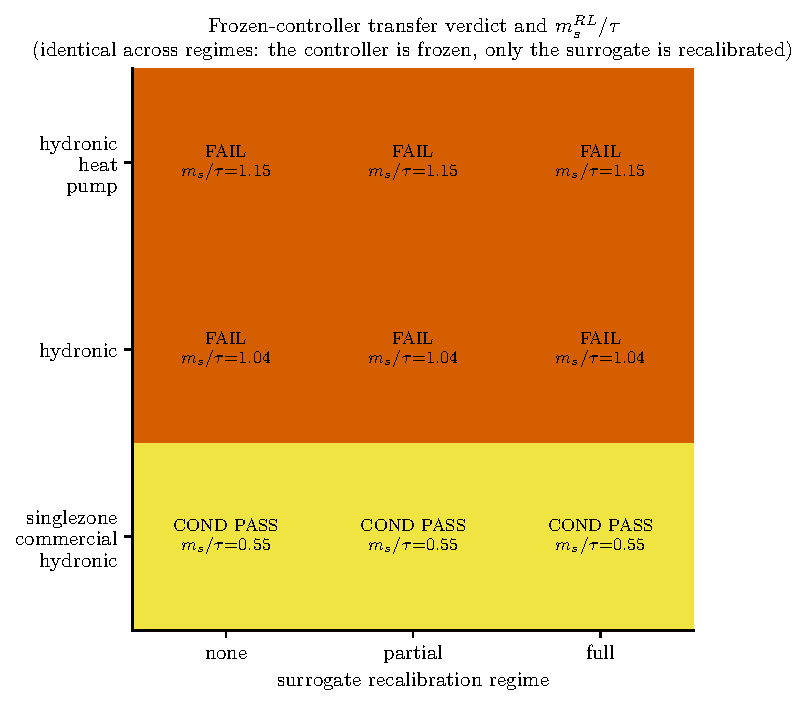
\includegraphics[width=0.84\linewidth]{final17_fig13_block3_controller_transfer_heatmap.pdf}
  \caption{Controller-transfer verdict heatmap. Residential hydronic cases fail the controller threshold; the commercial case passes the threshold but carries a separate energy caveat.}
  \label{fig:heatmap}

{\footnotesize\itshape Data: \texttt{reports/\allowbreak block3\_\allowbreak transfer\_\allowbreak matrix.csv}}
\end{figure}

\begin{figure}[H]
  \centering
  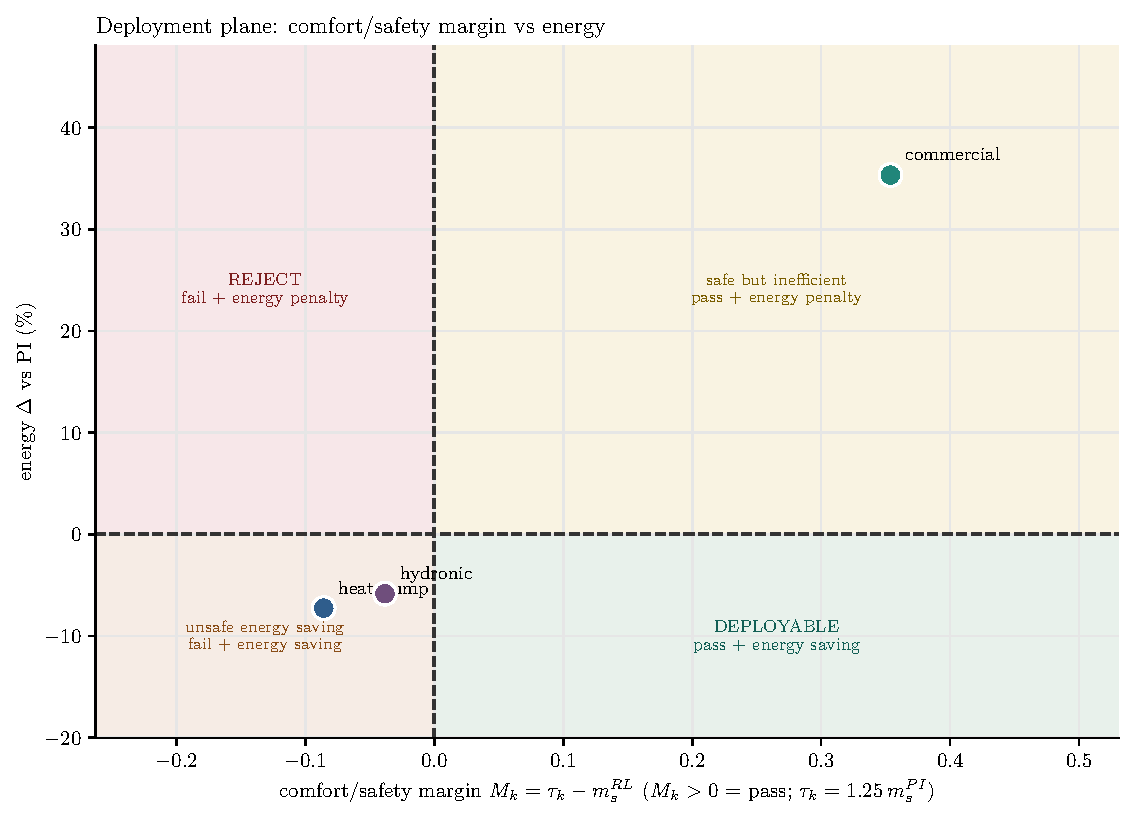
\includegraphics[width=0.84\linewidth]{block3_q1_polish_deployment_quadrants.pdf}
  \caption{Comfort--energy deployment plane. The residential cases save energy but fail the comfort/safety threshold; the commercial case passes the threshold but moves into the energy-penalty quadrant.}
  \label{fig:deployment_plane}

{\footnotesize\itshape Data: \texttt{reports/\allowbreak block3\_\allowbreak transfer\_\allowbreak matrix.csv}}
\end{figure}

\begin{figure}[H]
  \centering
  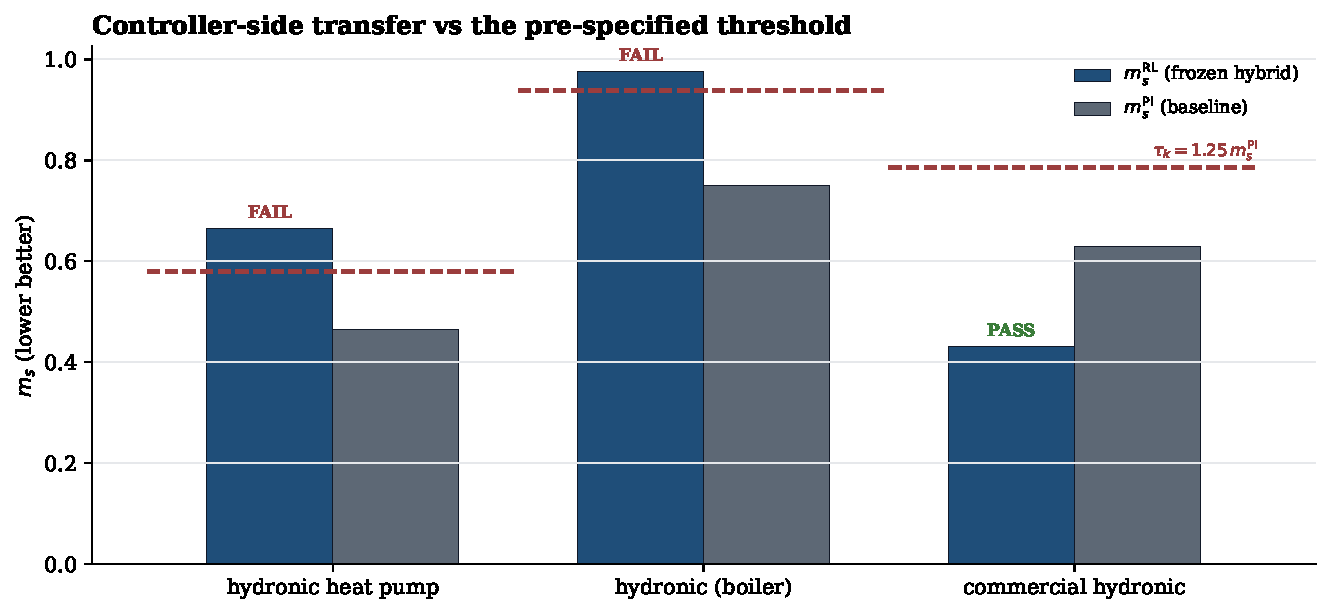
\includegraphics[width=0.80\linewidth]{fig_block3_controller_bar.pdf}
  \caption{Controller-side transfer: frozen-hybrid $m_s^{\mathrm{RL}}$ against the PI baseline $m_s^{\mathrm{PI}}$ and the pre-specified threshold $\tau_k=1.25\,m_s^{\mathrm{PI}}$ (dashed). The two residential cases exceed the threshold (FAIL); the commercial case is below it (PASS, with the separate energy caveat).}
  \label{fig:controller_bar}

{\footnotesize\itshape Data: \texttt{reports/\allowbreak block3\_\allowbreak transfer\_\allowbreak matrix.csv}}
\end{figure}

\subsection{Primary testcase: \texttt{bestest\_hydronic\_heat\_pump}}

The primary testcase was pre-specified as the easiest target (closest to \texttt{bestest\_air} in envelope class, but with a hydronic heat-pump actuator). The yearly PI baseline is $m_s=0.464$ with threshold $\tau=0.579$. The frozen hybrid controller obtains $m_s=0.665$ with energy $-7.3\%$ relative to PI, so the controller verdict is FAIL: the policy saves energy but violates comfort too often. Full Stage A/B/C recalibration instead succeeds (Table~\suppref{S17}): RMSE$_T=0.565\,^\circ$C and $C_{\mathrm{zon}}=8.348\times10^5$ J/K $=1.892\times$ \texttt{bestest\_air}. The component-level split is explicit: surrogate recalibration transfers; the frozen controller does not.





\subsection{Secondary testcase: \texttt{bestest\_hydronic}}

The secondary testcase tests whether the primary failure was specific to heat-pump nonlinearities. It was not. The residential boiler/radiator case has PI $m_s=0.750$ and threshold $\tau=0.938$; the frozen hybrid controller obtains $m_s=0.976$ with energy $-5.8\%$ relative to PI --- replicating the residential controller-side failure (energy saved, comfort threshold not met). Full Stage A/B/C again succeeds: RMSE$_T$ drops from $2.666$ to $0.335\,^\circ$C (a $87.4\%$ gain) and $C_{\mathrm{zon}}=1.954\times$ \texttt{bestest\_air}. The N=2 residential pattern is therefore consistent: frozen-controller transfer fails; surrogate recalibration transfers.

\subsection{Stretch testcase: \texttt{singlezone\_commercial\_hydronic}}

The stretch testcase was pre-specified as the hardest, most informative falsification probe. The manifest predicted that mode=none controller transfer would FAIL (a-priori probability 0.80) and that the commercial-scale $C_{\mathrm{zon}}$ would likely be scale-dependent (hypothesis B, $[3,10]\times$, a-priori 0.50). The observed result is mixed and scientifically useful. The frozen controller obtains $m_s=0.431$ against PI $m_s=0.628$ and threshold $0.785$, so it \emph{passes} the $m_s$ criterion --- but it consumes $35.3\%$ more energy than PI, so the correct reading is threshold PASS, not deployment-ready PASS. The surrogate side is again strong: full Stage A/B/C reduces RMSE$_T$ from $1.952$ to $0.238\,^\circ$C ($87.8\%$), and the identified $C_{\mathrm{zon}}$ ratio is $1.909\times$ --- inside the lower-probability uniform hypothesis A, not the predicted $3$--$10\times$ range.

\subsection{Surrogate-side transfer and $C_{\mathrm{zon}}$ consistency}
\label{ssec:czon}

Full Stage A/B/C improves target rollout RMSE on all three testcases (gains $60.2\%$, $87.4\%$, $87.8\%$), supporting the weak surrogate-side transfer hypothesis on $N=3$ (Figure~\ref{fig:stage_abc_gain}). The strongest physical finding is the consistency of the re-identified capacitance: the three hydronic testcases cluster tightly around $1.918\times$ the \texttt{bestest\_air} value (Table~\ref{tab:czon}),
\begin{equation}
  \rho_C = \{1.892,\,1.954,\,1.909\},
  \qquad
  \bar\rho_C = 1.918,\quad s_{\rho_C} = 0.032.
  \label{eq:czon_stats}
\end{equation}
The calibrated thermal capacitance is thus more closely associated with hydronic-family physics than with the obvious commercial zone-size proxy: despite the stretch testcase having an order-of-magnitude larger zone volume, its ratio sits within $\pm2\%$ of the family mean. This generalizes the calibration component of the v3.5 surrogate beyond a single building. The uniformity claim is, however, established on $N=3$ single-zone hydronic cases and is therefore a hydronic-family observation rather than a statistically powered law; it is not asserted for radiant, VRF, multi-zone, or cross-climate cases (Section~\ref{ssec:b3lim}).

\begin{table}[H]
\centering
\small
\caption{$C_{\mathrm{zon}}$ re-identification across the \texttt{bestest\_air} baseline and the three hydronic testcases (data: roadmap Section 15).}
\label{tab:czon}
\begin{tabular}{lrr}
\toprule
Testcase & $C_{\mathrm{zon}}$ (J/K) & $\rho_C$ vs \texttt{bestest\_air} \\
\midrule
\texttt{bestest\_air} (Block 1) & 4.413$\times10^5$ & 1.000 (baseline) \\
hydronic heat pump & 8.348$\times10^5$ & 1.892 \\
hydronic (boiler) & 8.623$\times10^5$ & 1.954 \\
commercial hydronic & 8.426$\times10^5$ & 1.909 \\
\midrule
hydronic-family mean $\pm$ std & --- & 1.918 $\pm$ 0.032 \\
\bottomrule
\end{tabular}
\end{table}

\begin{figure}[H]
  \centering
  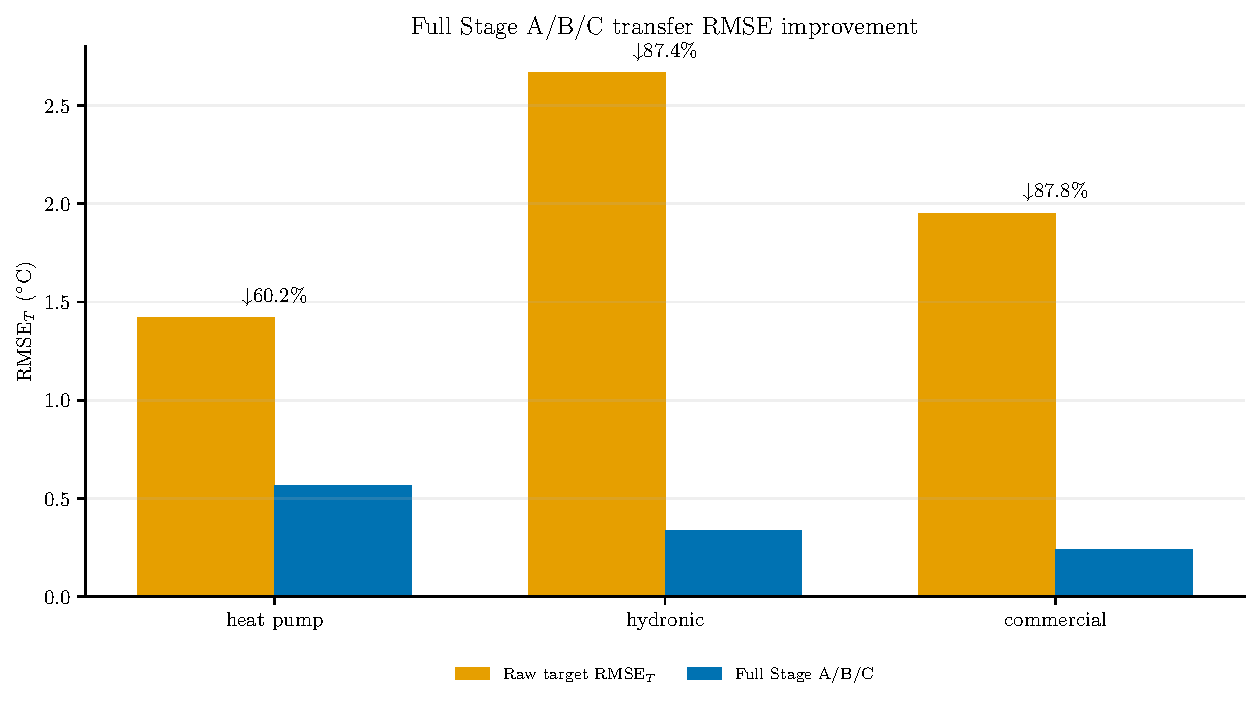
\includegraphics[width=0.84\linewidth]{final17_fig15_full_stage_transfer_rmse_improvement.pdf}
  \caption{Full Stage A/B/C transfer RMSE improvement on the three hydronic-family target testcases.}
  \label{fig:stage_abc_gain}

{\footnotesize\itshape Data: \texttt{reports/\allowbreak block3\_\allowbreak transfer\_\allowbreak matrix.csv}}
\end{figure}



\subsection{Hypothesis closure}

Table~\ref{tab:hypothesis} closes the pre-specified hypotheses. The methodological point is that Block 3 does not collapse the evidence into a single label: surrogate transfer and controller transfer diverge.

\begin{table}[H]
\centering
\small
\caption{Pre-specified hypothesis closure (manifest \texttt{hypothesis\_status\_final}, audit anchor \texttt{7ada793}).}
\label{tab:hypothesis}
\begin{tabularx}{\linewidth}{l >{\raggedright\arraybackslash}p{42mm} l >{\raggedright\arraybackslash}X}
\toprule
Hypothesis & Claim & Verdict & Evidence \\
\midrule
H1 (strong) & Frozen mode=none recipe gives deployment-ready transfer. & FALSIFIED & Residential cases fail the $1.25\times$ PI threshold; commercial is threshold-pass only with $+35.3\%$ energy. \\
H2 (medium) & Partial Stage C recovers controller transfer. & FALSIFIED (structural) & Partial recalibrates only the surrogate; the controller is frozen by scope, so live KPI cannot change. \\
H3 (surrogate) & Full Stage A/B/C gives a usable target surrogate. & SUPPORTED (N=3) & RMSE$_T$ gains 60.2\%, 87.4\%, 87.8\%; $C_{\mathrm{zon}}$ re-identified consistently. \\
H3 (controller) & Frozen controller transfers given a valid adapter. & FALSIFIED & Residential cases fail comfort; commercial passes safety but overuses energy --- regime-dependent failure. \\
hierarchy & Verdict is monotone in recalibration depth. & SUPPORTED & Controller KPI invariant under surrogate-only recalibration; surrogate fidelity improves with full recalibration. \\
\bottomrule
\end{tabularx}
\end{table}

\begin{figure}[H]
  \centering
  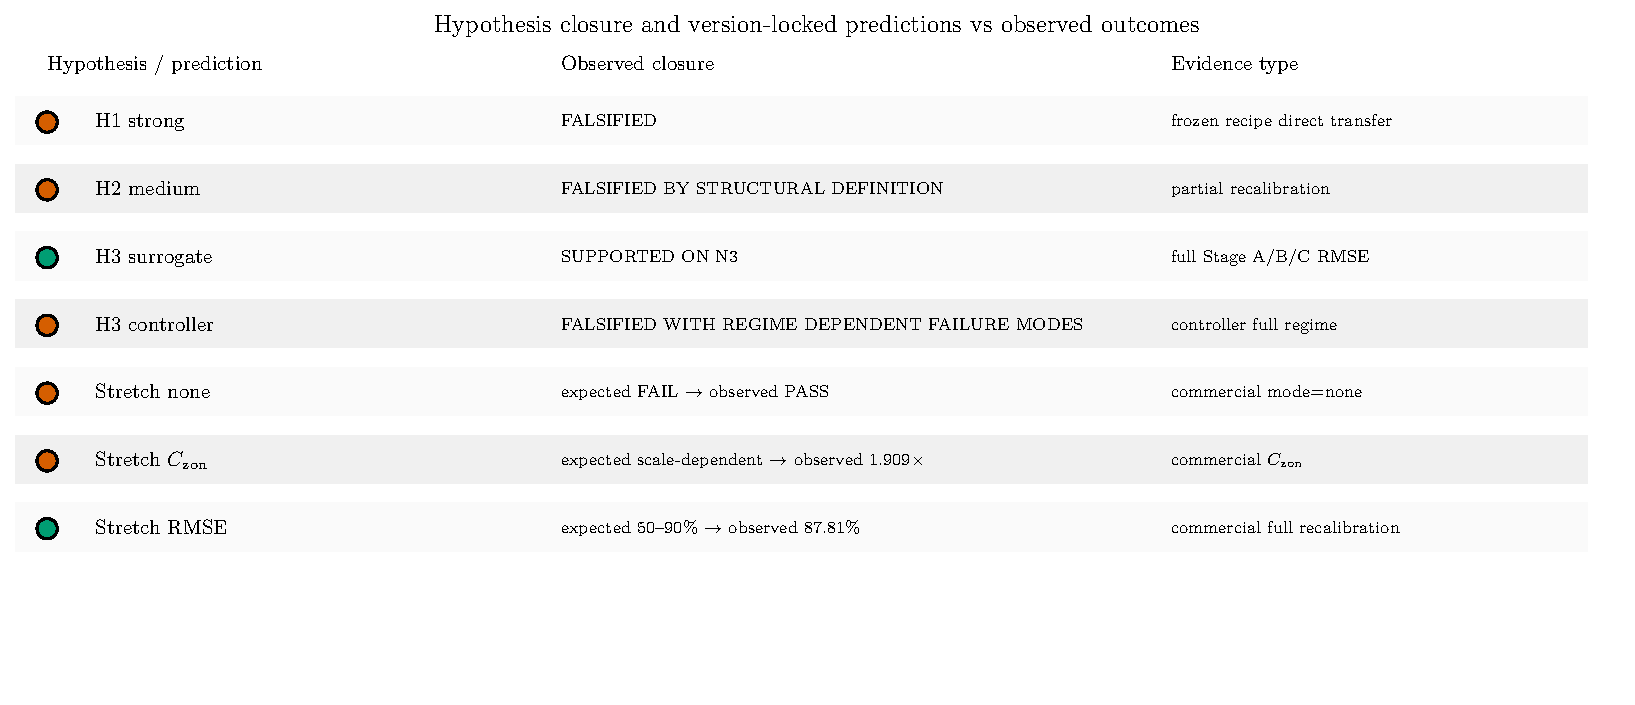
\includegraphics[width=0.88\linewidth]{final17_fig17_hypothesis_closure_matrix.pdf}
  \caption{Hypothesis closure matrix: Block 3 supports surrogate-side transferability but falsifies deployment-ready frozen-controller transfer.}
  \label{fig:hypothesis_closure}

{\footnotesize\itshape Data: \texttt{reports/\allowbreak block3\_\allowbreak transfer\_\allowbreak matrix.csv}}
\end{figure}

\subsection{Pre-specified predictions versus outcomes}

The stretch testcase carried numerical a-priori predictions (audit anchor \texttt{645626e}, logged before any commercial-hydronic run). Reporting the predicted-vs-observed mapping is the central Popperian discipline of Block 3 (Table~\suppref{S18}): the evidence moved the interpretation toward lower-prior hypotheses rather than confirming only what was expected. Two predictions were falsified (the mode=none controller FAIL, and the scale-dependent $C_{\mathrm{zon}}$ hypothesis) and three were confirmed.




\section{Discussion}\label{sec:discussion}

Before discussing the results in detail we separate the paper's primary claim from
its secondary findings, because they rest on different strengths of evidence. The
\emph{primary} claim is the fidelity--utility paradox and its mechanism: on the
\texttt{bestest\_air} testcase, increasing a surrogate's predictive fidelity can
remove the temporal smoothing that makes it a useful policy-gradient training
substrate. This claim is the load-bearing contribution and carries the strongest
evidence --- three matched-configuration comparisons scored on the live emulator
(direct v3.5, the matched-resolution v3 ablation of
Section~\ref{sec:results2-control}, and the canonical hourly v3), which together
isolate the fidelity/smoothing trade-off from the surrogate model class. The
remaining results are \emph{secondary}: they operationalise or bound the primary
claim rather than establish it. The hybrid role-separation recipe and the
controller-family-specific censor weight show \emph{one} engineering resolution of
the paradox; the MORL preference and seed-stability analysis characterises a third
controller family under a deliberately narrowed, audit-protected claim; and the
transferability study reports a component-level boundary on a hydronic family. These
secondary findings rest on narrower evidence (single-seed mechanistic comparisons, a
single PI baseline, simulation only) and are framed accordingly; the limitations that
bound each are collected in Section~\ref{ssec:b3lim}. A reader interested only in the
core result can read Sections~\ref{sec:results1-digital-twin}--\ref{sec:results2-control}
and the first subsection below; the transferability and MORL material extends rather
than supports the central paradox.

\subsection{Predictive validity versus RL training utility}
The central finding is that predictive fidelity and training utility are distinct,
and over part of the range opposed. The calibrated physical twin v3.5 is the better
predictor by a wide margin --- a 24-hour rollout \RMSE{} of $0.644\,^{\circ}$C
against $1.557\,^{\circ}$C for the black-box v3 --- yet used directly as the
training environment it produces an unusable controller ($m_s = 1.046$ live, comfort
violation above $77\%$), whereas the weaker v3 yields a usable one
($m_s = 0.073$/$0.095$). This inverts the working assumption of the surrogate
literature, whose protocols and accelerators are optimised for predictive accuracy
\citep{HouEvins2024} or raw throughput \citep{Mshragi2026FastML} on the implicit
premise that a better model is a better basis for control. Our matched-corpus
ablation further shows the fidelity gain itself is only $25.4\%$ physical
calibration against $74.6\%$ data resolution, so even the predictive improvement is
mostly an artefact of sampling rate rather than physics. A direct closed-loop
control settles the obvious confound: retraining the \emph{same} black-box v3 at the
matched fifteen-minute resolution produces a strictly \emph{more accurate} predictor
yet an unusable training environment ($m_s = 1.14$/$1.21$ live, $>85\%$ comfort
violation; Section~\ref{sec:results2-control}, Table~\ref{tab:coarse_graining}), so
the operative variable in this comparison is the fidelity/smoothing trade-off induced
by temporal resolution, not merely the black-box versus grey-box parameterisation. We read the paradox as a
distribution-shift phenomenon \citep{Quinonero2009DatasetShift,RiahiSamani2026OOD}:
a policy that exploits the sharply physics-constrained surface of v3.5 saturates
into a near bang-bang law that does not survive transfer to the live plant. The
hybrid resolution --- v3 for smooth dynamics, a frozen v3.5 as a reward-shaping
censor --- recovers the best cross-window robustness ($m_s = 0.087$/$0.041$ on the
peak/typical windows): although pure v3 edges it on the peak-window score alone
($0.073$ vs $0.087$), the hybrid is the only backend with sub-$5\%$ comfort
violation on \emph{both} windows, the lowest typical-window score ($0.041$), and
lower energy than pure v3, all while retaining an $85\times$ training speed-up ---
the practical pay-off of separating the two roles rather than seeking one maximally
faithful model.

\subsection{Controller-family specificity of the physical censor}
The physics-regularisation recipe is not universal across controllers, which
falsifies the natural expectation that one censor weight should serve all agents.
The optimal disagreement weight is $\lambda_{\mathrm{temp}}=0.10$ for the
thermostatic PPO agent but $\lambda_{\mathrm{temp}}=0$ for both the hierarchical
controller and the $17$-dimensional MORL controller: the latter two already see
enough forecast and structural context that an external physical censor only
over-constrains them. This is consistent with the view that hierarchical and
preference-conditioned agents shape their own effective dynamics through temporal
abstraction or preference conditioning \citep{Bacon2017Options,Nachum2018HIRO,Liao2025HDRL,Byeon2025MaxMinMORL},
and it cautions against reporting a single ``best'' regularisation strength without
stating the controller family it was tuned on.

\subsection{The transferability boundary}
The transferability result is best read not as a failure of policy transfer but as
a \emph{bounded generalization} claim with a sharp, component-level boundary: the
calibration \emph{pipeline} transfers, the frozen \emph{policy} does not transfer
uniformly. Re-running the Stage~A/B/C inverse calibration on the hydronic family
reduces rollout \RMSE{} by $60.2$--$87.8\%$, and the (effective) zone capacitance
re-identifies as a near-uniform ratio ($\Czon$ scales by $1.918\pm0.032\times$ the
source value) even across an order-of-magnitude change in zone volume, so the
calibration recipe is portable in a precise, quantified sense. Frozen-policy
transfer, by contrast, is regime-dependent and we report its boundary explicitly:
the commercial single-zone hydronic stretch testcase \emph{passes} the
$1.25\times$ PI comfort-safety threshold but at a $35.3\%$ energy penalty relative
to the baseline, whereas the residential hydronic cases \emph{fail} the
comfort-safety threshold under zero-shot reuse. This is a sharper statement than
the usual ``transfer reduces training cost'' claim \citep{Hou2024MultiSource}: it
identifies \emph{what} transfers (the identified physics), \emph{what} does not
(the control law), and \emph{under which regime} a frozen controller remains safe
--- a deployment-relevant boundary rather than an aggregate transfer benefit.

\subsection{Methodological implications and positioning}
Three methodological points follow. First, the choice of \emph{training environment}
--- not only the algorithm --- determines the resulting policy, so surrogate design
should be evaluated by downstream control utility and not predictive accuracy
alone; this complements, rather than contradicts, accuracy-oriented surrogate
protocols \citep{HouEvins2024} and the forecast-augmentation results that improve
RL-HVAC control \citep{Gao2024Predictive}. Second, because the failure mode is a
distribution shift between surrogate and live plant, the live-plant score must be
the reported metric, and safe-exploration framing \citep{Garcia2015SafeRL} applies
even when training is entirely in simulation. Third, the commit-anchored, version-locked audit-
anchored protocol is what lets us state H1 and H3 as \emph{falsified} rather than
quietly dropped; binding each hypothesis to a versioned anchor before the runs is a
discipline we recommend for surrogate-trained control studies, where the
temptation to report only the favourable configuration is strong. Relative to the
broader DRL-for-HVAC literature, which still reaches real-building deployment only
rarely \citep{AlSayed2024Review} and typically benchmarks against rule-based or
guideline baselines \citep{Savino2025ASHRAE}, our contribution is less a new
controller than a corrected account of \emph{why} surrogate-trained controllers
succeed or fail.

\subsection{Threats to validity}\label{ssec:block1-limitations}\label{ssec:b3lim}
Several limitations bound these claims. (i)~The primary testbed is a single-zone
\texttt{bestest\_air} emulator; multi-zone coupling and richer HVAC topologies are
not exercised, and the transferability evidence covers a hydronic family rather
than an arbitrary building stock. (ii)~The surrogate models are validated on the
temperature channel, where the calibration metrics are strong; the heating-power
channel is reproduced less accurately and we treat it as a known limitation rather
than a validated output. (iii)~Two caveats bound the core paradox claim. First, its mechanism is established
\emph{in direction} only --- we observe action saturation and attribute it to
policy-gradient exploitation of flat-gradient regions, but a formal loss-landscape
analysis is future work; correspondingly, the paradox is demonstrated for PPO under
a matched training configuration --- we did not separately re-tune PPO for the v3.5
environment or test off-policy algorithms (e.g.\ SAC, TD3), so its generality across
RL algorithms is open. Second, the black-box v3 is trained at a one-hour step but
used at the fifteen-minute control step, raising the question of whether v3's
\emph{training} utility stems from its black-box nature or partly from this timestep
mismatch. We resolved this confound directly with a matched-config closed-loop
control, reported in full as the temporal-coarse-graining ablation of
Section~\ref{sec:results2-control} (Table~\ref{tab:coarse_graining}): the \emph{same}
black-box v3 retrained on the fifteen-minute corpus is a strictly \emph{more accurate}
predictor ($0.876\,^{\circ}$C vs $1.557\,^{\circ}$C 24\,h rollout RMSE) yet, trained
under the \emph{identical} pure-v3 recipe, \emph{collapses} on the live emulator
($m_s = 1.14$/$1.21$, $85.6$/$91.4\%$ comfort violation), comparable to the
direct-v3.5 failure and far worse than the hourly-trained controller
($m_s = 0.073$/$0.095$). v3's training utility is therefore attributable to its
\emph{coarser temporal resolution}, not to its black-box class alone: the same
architecture at the finer, more faithful resolution is an unusable training
environment. This sharpens the paradox into a
near-monotonic statement along the fidelity axis---the least accurate surrogate
(hourly v3) trains a usable controller, while the more accurate matched-resolution
v3 and the most accurate calibrated v3.5 both fail---and is consistent with the
distribution-shift mechanism above: higher-fidelity dynamics, whether from finer
resolution or physical calibration, present the sharper gradient surface that
policy-gradient search exploits into a non-transferable near-bang-bang law (a formal
loss-landscape characterisation of that surface remains the open item noted above).
(iv)~Statistical support is uneven
across controller families: the MORL results are reported over $N=5$ seeds with
explicit standard deviation and a 95\% confidence interval (for the neutral
preference, $m_s = 0.187\pm0.078$, CI $[0.090,0.284]$, whose entire interval lies
far below the PI score of $0.910$, so the improvement over PI holds across all five
seeds), whereas the thermostatic and hierarchical controllers are single
deterministic-seed evaluations on fixed 14-day targeted windows, for which
per-controller confidence intervals are accordingly not reported. (v)~The only
baseline is BOPTEST's built-in PI controller (its reference controller); this study
tests \emph{surrogate training utility}, not whether the controllers beat a tuned
MPC, rule-based controller, or ASHRAE Guideline~36 sequence, and that
stronger-baseline comparison is out of the present scope. (vi)~The censor weight for
the MORL controller ($\lambda_{\mathrm{temp}}=0$) is adopted by analogy with the
hierarchical-controller sweep rather than from an independent MORL sweep, so its
optimality for MORL is asserted, not demonstrated. (vii)~The observation interface
and the surrogate backend are not fully crossed: we report the MORL $5$D-versus-$17$D
ablation, but not every backend$\times$observation combination, so the attribution
between interface width and backend choice is only partial. (viii)~Evaluation is
entirely in simulation: no live-building deployment is claimed, and the sim-to-real
gap beyond BOPTEST remains open. These bounds motivate the Block~4 directions noted
in the conclusion.

\section{Conclusion}\label{sec:conclusion}
We asked whether a surrogate with higher predictive fidelity is automatically a
better environment in which to train a reinforcement-learning HVAC controller, and
tested the question across three controller families and a hydronic family of
transfer testcases under a commit-anchored, version-locked protocol. The answer is
no. Only the temporally coarse, hourly-trained black-box surrogate (v3) trains a
usable controller: the most accurate physical twin (v3.5; $0.644\,^{\circ}$C 24-hour
rollout \RMSE) collapses ($m_s = 1.046$, comfort violation above $77\%$), and the
\emph{same} black-box architecture retrained at the finer $900$\,s resolution becomes
a \emph{more} accurate predictor ($0.876\,^{\circ}$C) yet also fails as a training
environment ($m_s = 1.14$/$1.21$, violation above $85\%$) --- a fidelity--utility
paradox (H1 falsified) whose operative variable is the fidelity/smoothing trade-off
induced by temporal resolution, not the surrogate model class; a matched-corpus
attribution further splits the predictive gain into $74.6\%$ data-resolution and only
$25.4\%$ physical calibration. Separating the two roles resolves it: using the
black-box surrogate for smooth rollout dynamics and a frozen physical twin as a
reward-shaping censor (H2 supported) recovers the best cross-window robustness of the
study ($m_s = 0.041$ typical, violation below $5\%$) at an $85\times$ training
speed-up. The censor strength is controller-family specific
($\lambda_{\mathrm{temp}}=0.10$ for thermostatic PPO, $0$ for the hierarchical and
MORL agents; H3 falsified), and transferability resolves into a component-level
boundary (H4): the inverse-calibration pipeline transfers --- rollout \RMSE{} falls
by $60.2$--$87.8\%$ and the zone capacitance re-identifies as a near-uniform
invariant ($1.918\pm0.032\times$ the source) --- whereas the frozen control policy
does not transfer zero-shot. The contribution is therefore less a new controller
than a corrected, quantified account of why surrogate-trained controllers succeed
or fail, together with a reusable role-separating recipe.

Several directions (the project's Block~4) follow directly from the limitations of
Section~\ref{ssec:b3lim}: extending the study from a single zone to multi-zone and
mixed-topology buildings; a formal loss-landscape analysis to turn the
hypothesised flat-gradient mechanism of the paradox into an established one;
improving the heating-power channel of the surrogate so it is a validated rather
than an auxiliary output; broadening transfer beyond the hydronic family and
pairing the transferable calibration pipeline with light policy adaptation instead
of zero-shot reuse; and, ultimately, closing the remaining sim-to-real gap through
deployment on a physical building.

\section*{CRediT authorship contribution statement}
% TODO: list every author with their CRediT roles; placeholder for the corresponding author below.
\textbf{Author One:} Conceptualization, Methodology, Software, Validation, Formal analysis, Investigation, Data curation, Writing -- original draft, Writing -- review and editing, Visualization.

\section*{Declaration of competing interest}
The authors declare that they have no known competing financial interests or
personal relationships that could have appeared to influence the work reported in
this paper.

\section*{Funding}
This research did not receive any specific grant from funding agencies in the
public, commercial, or not-for-profit sectors. % TODO: replace if any funding applies.

\section*{Data availability}
The source code, configurations, trained controller checkpoints, calibration and
training data, result tables, and all artefacts required to regenerate the figures
and tables of this study are openly available on GitHub
(\url{https://github.com/Almaz-2001/HVAC_fidelity-utility-paradox}); the repository
will be archived with a citable DOI upon acceptance. Every reported quantity is
mapped to its source artefact by the per-section provenance tables (Supplementary
Tables~S1--S3). The BOPTEST emulator used as the reference environment is available
separately as part of the BOPTEST project \citep{Blum2021BOPTEST} at
\url{https://github.com/ibpsa/project1-boptest}.

\section*{Supplementary material}
Every figure, table, and inline number in Results~I--III is read directly from the
versioned \texttt{reports/} and \texttt{outputs/} artefacts. The separate
Supplementary Material document provides the complete content-to-artefact
provenance maps for the three evidence blocks (Supplementary Tables~S1--S3) together
with the parameter, configuration, and interface tables referenced from the main
text (Supplementary Tables~S4--S9).

\section*{Declaration of generative AI and AI-assisted technologies in the manuscript preparation process}
During the preparation of this work, the author(s) used Claude (Anthropic) to
assist with language editing, improving the readability and clarity of the text,
and with \LaTeX{} formatting and reference-list preparation. After using this tool,
the author(s) reviewed and edited the content as needed and take full responsibility
for the content of the published article. No generative AI tool was used to generate,
analyse, or interpret the research data, or to produce the scientific findings and
conclusions, which are the work of the author(s).

\section*{Acknowledgements}
% TODO: add any people/institutions to thank, or state "None.".
The authors thank the developers of the open-source BOPTEST framework. % adjust as needed.

\bibliographystyle{unsrtnat}
\bibliography{references}

\end{document}
